\documentclass[10pt]{article}

%%%%%%%%%%%%%%%%%%%%%%%%%%%%%%%%%%%%%%%%%%%%%
% Package Inclusion and Document Formatting %
%%%%%%%%%%%%%%%%%%%%%%%%%%%%%%%%%%%%%%%%%%%%%
\usepackage
{geometry,amsmath,amsthm,mathrsfs,amssymb,graphicx,bm,hyperref,url,pdfsync,
fancyhdr}
\pagestyle{fancy}
\numberwithin{equation}{section}
%%%%%%%%%%%%%%%%%%%
% Custom Commands %
%%%%%%%%%%%%%%%%%%%
\newcommand{\n}{\noindent}
\newcommand{\norm}[1]{\left\lvert#1\right\rvert}
\newcommand{\avg}[1]{\left\langle#1\right\rangle}
\newcommand{\abs}[1]{\left\vert#1\right\vert}
\newcommand{\figref}[1]{Figure \ref{#1}}
%%%%%%%%%%%%%%%%%%%%%%%%%%
% Title Page Information %
%%%%%%%%%%%%%%%%%%%%%%%%%%

\title{Notes for PHYS 234: High Energy Astrophysics}
\author{Bill Wolf}
\date{\today}

\begin{document}

\vfill\maketitle\vfill \newpage

\tableofcontents \newpage

%%%%%%%%%%%%%%%%%%%%%%
% April 1, 2013 %
%%%%%%%%%%%%%%%%%%%%%%

\section{Introduction} % (fold)
\label{sec:introduction}
	\emph{Monday, April 1, 2013}\\
	\subsection{What is High Energy Astrophysics?} % (fold)
	\label{sub:what_is_high_energy_astrophysics_}
	There are many definitions, but one is that high energy astrophysics is ``the study of the violent and extreme processes in the universe.'' Another traditional definition is the study of processes that produce gamma rays and X-rays (possibly ultraviolet radiation as well). Unfortunately, such high energy photons are very effectively blocked by the Earth's atmosphere, so observations are limited to being taken from the upper atmosphere or space. As a result, high energy astrophysics is a relatively young subfield of astrophysics ($\lesssim 100\ \mathrm{yrs}$).\\
	
	\n For our purposes, we will take an expanded view of what high energy astrophysics is, including white dwarfs (WDs), supernovae (SNe), and other phenomena.
	% subsection what_is_high_energy_astrophysics_ (end)
	\subsection{How is the High Energy Sky Different?} % (fold)
	\label{sub:how_is_the_high_energy_sky_different_}
	In this course, we will deal with energy in terms of electron volts (eV). A common photon energy of interest to us has an energy of 1 MeV, which is roughly equivalent to 1 million optical photons (which are thus obviously about 1 eV in energy). If we fix energy, high energy (HE) events must produce fewer photons since each is carrying more energy. In addition to smaller photon counts, HE events are rarer, so there are far fewer sources in the sky at any given moment. There are on the order of $10^5$ bright X-Ray sources (detectable by Chandra), on the order of $10^3$ bright gamma ray objects (detectable by Fermi), about 50 events that are bright around 100 MeV, and dozens of objects with energies of TeVs. Additionally, we observe catastrophic fast and transient events that are here and gone again.
	
	%
	% X-Ray and gamma-Ray map figures
	%
	% subsection how_is_the_high_energy_sky_different_ (end)
	
	\subsection{High Energy Photons} % (fold)
	\label{sub:high_energy_photons}
		Traditionally  $0.1\ \mathrm{keV} - 100\ \mathrm{TeV}$ constitute ``high energy photons''.
		\begin{table}[b]
			\centering
			\begin{tabular}{l l l}
				Symbol & Value & Units\\
				\hline
				$h$ & $6.626\times 10^{-27}$ & $\mathrm{erg\,s}$\\
				$1\,\mathrm{eV}$ & $1.602\times 10^{-12}$ & $\mathrm{erg}$\\
				1 \AA & $10^{-8}$ & cm\\
				$r_{\mathrm{proton}}$ & $\sim 10^{-13}$ & cm
			\end{tabular}
			\caption{Essential units in HE Astrophysics}
			\label{tab:1}
		\end{table}
		Some basic units are presented in Table~\ref{tab:1}. Related to those, a few other relations of interest are presented in Table~\ref{tab:2}.
		\begin{table}[b]
			\centering
			\begin{tabular}{l l l}
				Symbol & Value & Units\\
				\hline
				1 erg & 624 & GeV\\
				$m_ec^2$ & 511 & keV\\
				$m_pc^2$ & 931 & MeV\\
				1 keV / $k$ & $11.6\times 10^6$ & K\\
				1 keV / $c$ & $242\times 10^{17}$ Hz
			\end{tabular}
			\caption{Additional energy scales}
			\label{tab:2}
		\end{table}
		As we'll see, the messengers of HE processes are all over the EM spectrum, particularly at radio wavebands. Additionally, neutrinos, particles, and gravity waves get in the mix, giving rise to the phrase ``multi-messenger'' astrophysics.
	% subsection high_energy_photons (end)
	\subsection{History} % (fold)
	\label{sub:history}
		R\:{o}ntgen discovered X-rays in 1895, earning him the Nobel prize in 1901. In 1914, Henry Moseley developed the use of spectroscopy for HE processes through Moseley's Law in 1914. A bit earlier, Victor Hess discovered cosmic rays (1912) through the use of balloon experiments. He found that there was more ionization farther from Earth, indicating a new as of yet undiscovered source of ionizing radiation, earning him the Nobel Prize in 1936. In 1962, Giacconi used sounding rockets to contribute significantly to the study of X-rays. In particular, he discovered Sco X-I. His efforts in X-Ray astronomy earned him the Nobel prize in 2002.\\
		
		\n In 1977, the first X-ray satellite went into orbit, HEAO-I, which had a bandwidth of 0.2 keV - 10 MeV. It detected 842 discrete sources. Later HEAO-2 (later renamed Einstein) was launched with a bandwidth of 0.1 keV - 20 keV. This was the first X-ray telescope capable of focussing incoming radiation. In 1992, the Compton Gamma Ray Observatory (CRGO) was launched. It allowed gamma ray bursts to be localized. Previously, gamma ray bursts were of unknown origins. In 1999, Chandra was launched, which is also able to focus X-Rays. More recently, Fermi was launched in 2008, which is a gamma ray focusing telescope. Of particular interest is the LAT (Large Area Telescope) which allows detections of extremely high energy photons. To date, the newest satellite is NuStar, which was launched in 2012 and excels in spectroscopy of high energy sources.
	% subsection history (end)
	\subsection{X-Ray Spectra and Moseley's Law} % (fold)
	\label{sub:x_ray_spectra}
		The \emph{continuum} in X-Ray sources is caused by Bremsstrahlung ``braking radiation'' (free-free). Essentially an electron scatters off a proton and emits an X-ray in the process. The \emph{lines} in the spectra are \textbf{K-shell} emissions. This is similar to H$\alpha$ emission, but on heavier elements. Essentially, an electron from a low shell is ejected, allowing a higher $n$ electron to fall to the ground ($K$) shell, emitting in the X-ray.\\
		
		\n Moseley's Law states that the shell energy scales like the atomic number to the second power. It is then analogous to the Bohr atom ($\mathrm{K}\alpha\sim\mathrm{H}\alpha$). Transition energies are then given by
	\begin{align}
		\label{eq:1} h\nu &= 13.6\,\mathrm{eV}(Z-1)^2\left[\frac{1}{n_f^2}-\frac{1}{n_i}^2\right]\\
		\label{eq:2}      &= 13.6\,\mathrm{eV}(Z-1)^2\left[\frac{1}{1}-\frac{1}{2^2}\right]
	\end{align}
	Equation \eqref{eq:2} is the K$\alpha$ line for a ion with atomic number $Z$ with an $n=1$ electron kicked out ahead of time. This law accurately reflects the energies of lines we observe in X-Ray spectra.
	% subsection x_ray_spectra (end)
	\subsection{Detectors} % (fold)
	\label{sub:detectors}
		There are three main ways to stop HE photons
		\begin{enumerate}
			\item[1.] Photoelectric absorption: 
			\begin{equation*}
				\gamma + \mathrm{atom} \to \mathrm{atom}^+ + e^-
			\end{equation*}
			\item[2.] Compton Scattering:
			\begin{equation*}
				\gamma + e^- \to \gamma + e^-
			\end{equation*}
			This is essentially the high energy limit of Thomson scattering which allows for energy transfer
			\begin{figure}[h]
				\centering
				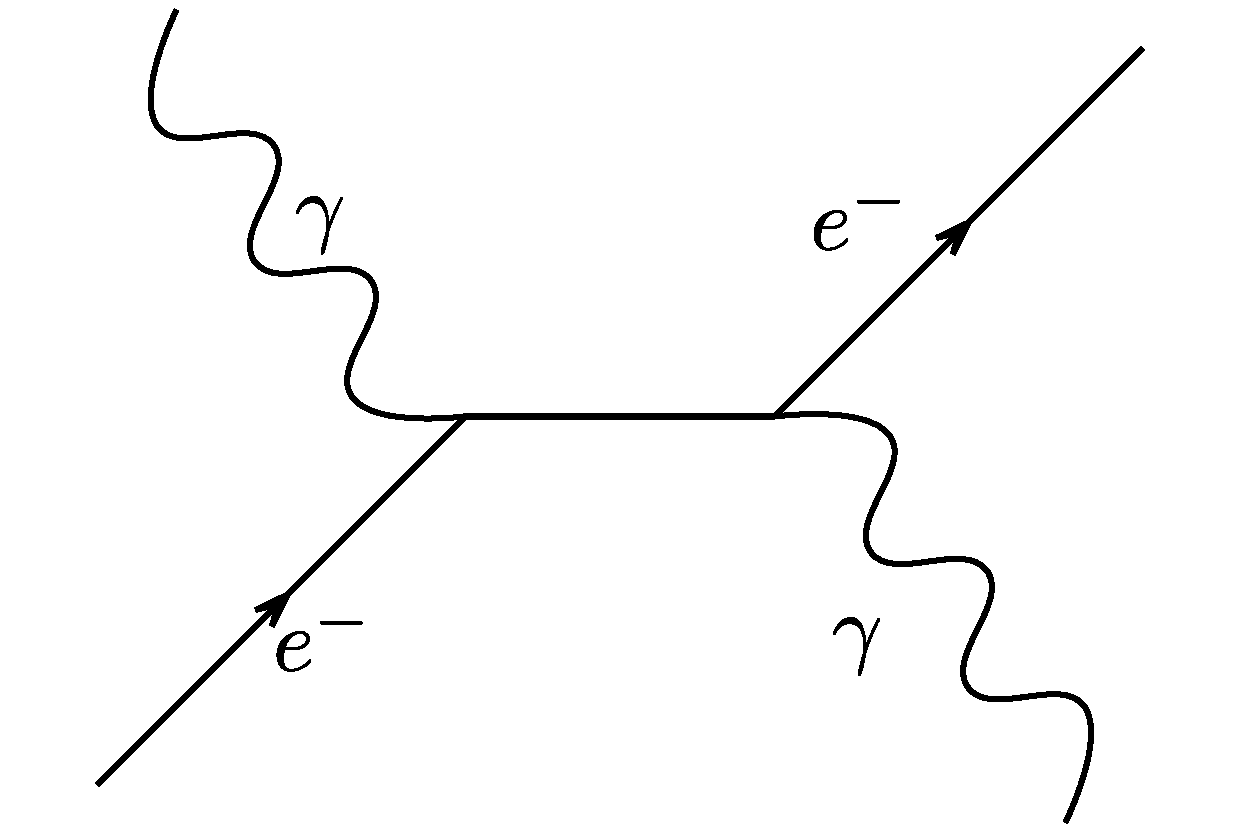
\includegraphics[width = 2in]{figures/compton_scatter.pdf}
				\caption{Schematic of Compton Scattering}
				\label{fig:1}
			\end{figure}
			\item[3.] Pair Production
			\begin{equation*}
				\gamma + \mathrm{nucleus} \to e^+ + e^- + \mathrm{nucleus}
			\end{equation*}
			The nucleus is required to appease conservation laws
		\end{enumerate}
		All three of these have been used to make HE photon detectors since they can generate measurable electrons. To characterize the absorption of photons in a material through some characteristic wavelength $\ell$, we'll assume there is some initial intensity $I$ of HE photons. This intensity if attenuated according to
		\begin{equation}
			\label{eq:3} I = I_0 e^{-\left(\frac{\mu}{\rho}\right)\rho \ell}
		\end{equation}
		where $\rho$ is the density of the material and $\mu/\rho$ is the ``mass attenuation'' (similar to an opacity), given by
		\begin{equation}
			\label{eq:4} \frac{\mu}{\rho} = \underbrace{\frac{\sigma}{\rho}}_{\mathrm{Compton}} + \underbrace{\frac{\tau}{\rho}}_{\mathrm{photoelectric}} + \underbrace{\frac{\kappa}{\rho}}_{\mathrm{pair\ production}}
		\end{equation}
		Knowing how your detector material is sensitive to each of the HE photon stoppage sources is essential to designing an effective HE photon telescope. Now we'll discuss some different types of HE detectors.\\
		
		\n \textit{Wednesday, April 3, 2013}\\
		
		\begin{table}[b]
			\centering
			\begin{tabular}{llp{3in}}	
			Energy & $T_{\mathrm{thermal}}$ & Process\\
			\hline
			$< 10\,\mathrm{keV}$ & $< 10^8\ \mathrm{K}$ & $K$ and $L$ shell line emission, Bremsstrahlung, thermal blackbody\\
			$10\,\mathrm{keV} - 10\,\mathrm{MeV}$ & - & non-thermal processes: isomeric transitions from metastable isomers (gamma ray lines), e.g. ${}^{60}\mathrm{Co} \to {}^{60}\mathrm{Ni}+e^- + \bar{\nu}_e + 1.15\,\mathrm{MeV}$ (present in supernova remnants)\\
			$511\,\mathrm{keV}$ & $10^9\ \mathrm{K}$ & $m_ec^2$ annihilation lines (seen in galactic center). E.g. $e^-+e^+ \to \gamma+\gamma$\\
			$140\ \mathrm{MeV} - 10\ \mathrm{GeV}$ & $10^{12}\ \mathrm{K}$ & Pion decay (strong force)\\
			$>10\ \mathrm{GeV}$ & - & non-thermal processes: inverse Compton scattering, shock acceleration
			\end{tabular}
			\caption{Different sources of high energy photons.}
			\label{tab:3}
		\end{table}
		
		\paragraph{Gas Proportional Counters} A gas of Argon and (other stuff?) absorbs HE photons, which then give off free electrons which are collected and counted. This is essentially Geiger counter. Each interaction causes multiple ionizations, so we are able to detect individual photons.
		
		\paragraph{Scintillation Counters} This detector relies on a crystal with doping, providing so-called ``actuator sites''. Incoming photons create an electron-hole pair which gets re-radiated at the actuator site around 4200\AA. This process is about 12\% efficient. The produced light then interacts with a photomultiplier tube.
		
		\paragraph{Solid State} Solid State detectors function much like CCDs from optical astronomy, but using materials that are better suited to HE photons.\\
		
		\n These detectors will count HE photons, but they do not provide directional information, like a camera with no telescope. So now we'll talk about different telescopes used for HE astrophysics. One big problem in such telescopes is that focussing is very difficult. In deed, HE photons will pass through mirrors unless glancing at an angle of three degrees or less. In 1952, Wolter came up with a way to effective focus X-rays using a barrel of parabolic and hyperbolic mirrors to gradually focus the X-rays through a series of many gentle reflections. As an example, NuStar will use 130 concentric mirrors to focus X-rays with energies as high as 79 keV. Chandra, XMM, HEAO-2/Einstein all work in this manner. Parabolic mirrors would focus an image onto a point, so hyperboloids are employed to focus images onto a plane, giving a field of view.\\
		
		\n At higher energies, HE astronomers use \textbf{coded aperture masks}. These devices have a pattern of transparent and opaque partitions which will project different observed patterns at different angles. These differing patterns can be analyzed to reproduce an image. This technology is used by HETE-2, Swift, and Integral.\\
		
		\n Additionally, we use Compton scattering and pair production devices to detect very high energy photons. Here, a gamma ray can interact with a Tungsten foil, causing pair production, which can be detected via a calorimeter. This is how the LAT instrument on Fermi works.\\
		
		\n At the very highest energies, we must go back to the ground in order to use air showers. Such instruments include HESS, CANGAROO, and VRITAS. Here, a cosmic ray interacts with the air, moving faster than the local speed of light. This in tern, causes a cone of Cerenkov radiation. With an array of detectors, the air shower can be detected and the angle of the cone can be ascertained, giving the energy of the cosmic ray. Typically we get 100 optical photons per square meter for each 100 GeV photon. \\
		
		\n Note that, beyond photons, HE processes produce other objects of interest. \textbf{Cosmic rays} are essentially high energy protons, electrons, nuclei, and other charged particles. Low energy neutrinos are produced through inverse beta decays ($p+e^- \to n+ \nu_e$). High energy neutrinos come from\ldots pion stuff ($\gamma+p \to n+\pi^+$, $\pi^+ \to \mu + \nu_\mu$). Finally, we can observe (ostensibly) gravity waves from rapidly changing gravitational fields.
	% subsection detectors (end)
	
	\subsection{Radioactivity} % (fold)
	\label{sub:radioactivity}
		In 1898, Henri Becquerel discovered radioactivity by examining how uranium salts interacted with photographic plates. The actual term ``radioactive'' was coined by Marie and Pierre Curie. It was Rutherford in 1899 who first came up with the nomenclature of $\alpha$, $\beta$, and $\gamma$ rays, which are ordered in increasing penetration capability. Now we know that they are completely different things: helium nuclei, electrons, and\ldots well\ldots $\gamma$-rays.
	% subsection radioactivity (end)
	
	\subsection{Energetics} % (fold)
	\label{sub:energetics}
		In stellar evolution, we learn that gravitational energy is not a primary source of energy except in early formation and late collapse phases. Even in the core collapse scenario, most of the gravitational energy is lost in the form of neutrinos. In general, then, gravitational binding energy release is unimportant to most stars most of the time. Other scales of energy release can be important though.\\
		
		\n Chemical reactions give only a few eV per baryon. For instance 10 eV per baryon corresponds to $10^{13}\ \mathrm{erg/g}$. Chemical processes are not really important in astronomy as energy sources.\\
		
		\n Nucleosynthesis, on the other hand, gives about 1 MeV per baryon, equivalent to $10^{18}\ \mathrm{erg/g}$. Note that the greatest gains in nucleosynthesis come from the simplest steps (like hydrogen to helium). Higher burning gives less and less energy, and eventually at Iron, there are no more energy gains to be had. \\
		
		\n Accretion power is more efficient still since it scales as $GM/R$. For the sun, this corresponds to about $2\times 10^{15}\ \mathrm{erg/g}$. One proposed explanation for the energy source for the sun was gravitational contraction. If we take the gravitational energy of the sun and divide by its current luminosity, we get a lifetime on the order of $10^{7}\ \mathrm{years}$-- far too short to account for how long it has been shining on Earth. Quasi-stellar objects (QSOs), on the other hand, are powered by the accretion of matter (not nuclear powered!). We observe them at $L_{\mathrm{QSO}}\sim 10^{47\ \mathrm{erg/s}}$. If this was powered by nuclear reactions, there would need to be about $10^{12}\ \mathrm{M_\odot}$ of matter burned each Gyr to provide the power! Mass estimates for these objects are only as high as $10^{11}$, so they are likely powered by accretion.
	% subsection energetics (end)
% section introduction (end)
\section{Accretion of Astrophysical Plasmas} % (fold)
\label{sec:accretion_of_astrophysical_plasmas}
	\subsection{Spherical Flow onto Compact Objects} % (fold)
	\label{sub:spherical_flow_of_ionized_material_onto_compact_objects}
		Now we will consider the spherically symmetric accretion of matter onto a compact object. This essentially ignores angular momentum, which will be included at a later time when we discuss accretion disks.\\
		
		\n There is a fundamental limit on the rate at which matter can be accreted, called the \textbf{Eddington Limit}.\\
		
		\n\emph{Monday, April 8, 2013}\\
		
		% Monday, April 8, 2013
		\n This limiting accretion rate is achieved when outward radiation pressure is perfectly balanced with inward gravity. Consider a fully-ionized medium of pure hydrogen (protons and electrons) The gravitational force for a given particle is 
		\begin{equation}
			\label{eq:acc:1} F_{\mathrm{grav}} \approx -\frac{GM(m_{\mathrm{particle}})}{r^2} \sim -\frac{GM m_p}{r^2}
		\end{equation}
		Now we'll define a number flux of photons at a particular frequency via
		\begin{equation}
			\label{eq:acc:2} S_\nu = \frac{L_{\mathrm{Edd}}}{4\pi r^2 h\nu}
		\end{equation}
		We'll assume that radiative transfer is dominated by Thomson scattering, which gives an effective cross section of
		\begin{equation}
			\label{eq:acc:3} \sigma_{\mathrm{T}} = \sum_i \frac{2}{3}\left(\frac{e_i^2}{m_i c^2}\right)^2
		\end{equation}
		Since the proton is $\sim 2000$ times more massive than an electron, the electron dominates the cross section. With this in hand, we want to find the force due to radiation pressure,
		\begin{equation}
			\label{eq:acc:4} F_{\mathrm{rad}} = \sigma_{\mathrm{T}}S_\nu p = \frac{\sigma_{\mathrm{T}}L}{4\pi r^2 c}
		\end{equation}
		where $p$ is the momentum of a photon with frequency $\nu$, namely $p=h\nu/c$. We can now solve for the Eddington Luminosity:
		\begin{equation}
			\label{ea:acc:5} L_{\mathrm{Edd}} = \frac{4\pi G m_p c M}{\sigma_{\mathrm{T}}}
		\end{equation}
		where we've set $F_{\mathrm{grav}}$ equal to $F_{\mathrm{rad}}$. Parameterizing to solar masses, this gives a luminosity of
		\begin{equation}
			\label{eq:acc:6} L_{\mathrm{Edd}} = 1.3\times 10^{38}\left(\frac{M}{M_\odot}\right)\,\mathrm{erg\ s^{-1}} = 6.5\times 10^{4}\left(\frac{M}{M_\odot}\right)\,L_\odot
		\end{equation}
		This it the fundamental luminosity of a star or accreting object. Luminosities higher than this would result in mass loss. If an object shining at the Eddington luminosity radiates as a blackbody, we can find a characteristic temperature (at a given radius and mass):
		\begin{equation}
			\label{eq:acc:7} T_{\mathrm{eff}} = \left(\frac{cGM m_p}{R^2\sigma_{\mathrm{T}}\sigma_\mathrm{B}}\right)^{1/4}
		\end{equation}
		For a neutron star, this corresponds to $kT\approx 1.9\ \mathrm{keV}$ and for a white dwarf, $kT\approx 53\ \mathrm{eV}$. This is essentially the shock energy of infalling particles of accreted matter.\\
		
		\n There is an effective accretion rate, $\dot{M}$ that corresponds to $L_{\mathrm{Edd}}$ if we assume that all of the luminosity is liberated at the edge of the star. The accretion luminosity is given by
		\begin{equation}
			\label{eq:acc:8} L_{\mathrm{acc}} \approx \frac{GM\dot{M}}{R}
		\end{equation}
		Equating this to the Eddington luminosity gives us the limiting accretion rate:
		\begin{equation}
			\label{eq:acc:9} \dot{M}_{\mathrm{Edd}} = \frac{4\pi m_p c R}{\sigma_{\mathrm{T}}}
		\end{equation}
		For a neutron star, this corresponds to $\dot{M}\sim 10^{-8}\,M_\odot/\mathrm{yr}$ and for a white dwarf, $\dot{M}\sim 10^{-5}\,M_\odot/\mathrm{yr}$. The accretion rate indicated by the capture rate of plasma by a central object must depend on properties at large distances as well as the mass of the central object. All other dynamics should be dictated by the background material as well as the pull of the large central mass.\\
		
		\n We then define $\rho(\infty)$ to be the density at a sufficiently large distance away from the central object. Similarly, $c_s(\infty)$ and $T(\infty)$ are the asymptotic sound speed and temperature, respectively. We'll assume material at this sufficiently far enough distance starts at rest with respect to the bulk plasma. The capture rate can be modeled to be
		\begin{equation}
			\label{eq:acc:9a} \dot{M} = \pi r_{\mathrm{cap}}^2 v_{\mathrm{eff}}\rho(\infty)
		\end{equation}
		where $r_{\mathrm{cap}}$ designates the radius to which the central mass is able to influence the background medium and $v_{\mathrm{eff}}$ is the effective velocity at the capture radius. If the particles are streaming by the mass, $r_{\mathrm{cap}}$ must be related to some typical velocity (for instance, the velocity of a passing wind). If at rest, though, $r_{\mathrm{cap}}$ is related to the sound speed, $c_{s}$. In fact, we know that $c_s^2$ is just the thermal energy per unit mass (up to a factor of two), so we may specify
		\begin{equation}
			\label{eq:acc:9b} c_s(\infty)\sim \sqrt{\frac{kT}{m_{\mathrm{H}}}} \sim 10\,\mathrm{km/s}\,\sqrt{\frac{T}{10^8\,\mathrm{K}}}
		\end{equation}
		Setting the asymptotic sound speed equal to the escape velocity, $c_s \sim \sqrt{GM/r_{\mathrm{cap}}}$, we find the capture radius for static plasma to be
		\begin{equation}
			\label{eq:9c} r_{\mathrm{cap}} = \frac{GM}{c_s^2(\infty)}
		\end{equation}
		Now identifying $v_{\mathrm{eff}}$ and $c_s(\infty)$, we arrive at an accretion rate
		\begin{equation}
			\label{eq:acc:10} \dot{M} \approx \frac{\pi G^2 M^2}{c_s^4(\infty)}c_s(\infty)\rho(\infty) = \frac{\pi G^2 M^2\rho(\infty)}{c^3_s(\infty)}
		\end{equation}
		To get some intuition, let's assume a number density of $n=1\ \mathrm{cm^{-3}}$, which corresponds to $\rho=1.6\times 10^{-24}\ \mathrm{g/cm^3}$, and a sound speed of $c_s=10^6\,\mathrm{cm/s}\sqrt{T/10^4\ \mathrm{K}}$. For a $1.4\,M_\odot$ neutron star, this give a capture rate of 
		\begin{equation}
			\label{eq:acc:11} \dot{M} = 1.8\times 10^{11}\,\mathrm{g/s}\,\left(\frac{M}{1.4M_\odot}\right)^2\left(\frac{n}{1\,\mathrm{cm^{-3}}}\right)\left(\frac{T}{10^4\,\mathrm{K}}\right)^{-3/2} \sim 10^{-15}\,M_\odot/\mathrm{yr}
		\end{equation}
	% subsection spherical_flow_of_ionized_material_onto_compact_objects (end)
	\subsection{A More Detailed Calculation} % (fold)
	\label{sub:a_more_detailed_calculation}
		Any treatment of accretion of plasma must satisfy the continuity equation (essentially mandating mass conservation), namely
		\begin{equation}
			\label{eq:acc:12} \frac{\partial \rho}{\partial t} + \bm{\nabla}\cdot (\rho\mathbf{v})=0
		\end{equation}
		In a steady state, the time derivative must vanish, leaving us with simply
		\begin{equation}
			\label{eq:acc:13}\bm{\nabla}\cdot(\rho\mathbf{v}) = 0
		\end{equation}
		$\rho\mathbf{v}$ is essentially the mass flux. Its divergence is the net flux of mass per unit volume (a positive value would mean mass is accumulating at point and a negative value would mean that mass is being depleted from a point). We will assume spherically symmetric inflow ($\mathbf{v} = -v\,\hat{r}$). The continuity equation then tells us
		\begin{equation}
			\label{eq:acc:14} \frac{1}{r^2}\frac{d}{dr}\left(r^2\rho v\right) = 0 \qquad \Rightarrow \qquad r^2\rho v = \mathrm{constant}
		\end{equation}
		We can also write down an accretion rate given the mass flux:
		\begin{equation}
			\label{eq:acc:15} \dot{M} = 4\pi r^2\rho v
		\end{equation}
		which allows us to eliminate the velocity via
		\begin{equation}
			\label{eq:acc:16} v = \frac{\dot{M}}{4\pi r^2\rho}
		\end{equation}
		In addition to conserving mass, we must conserve momentum, introducing the Euler equation:
		\begin{equation}
			\label{eq:acc:17} -\bm{\nabla}P + \mathbf{f} = \rho\frac{\partial{\mathbf{v}}}{dt} + (\rho\mathbf{v} \cdot \bm{\nabla}) \mathbf{v}
		\end{equation}
		where $\mathbf{f}$ is the external force density. Starting with the left side, we expand to get
		\begin{equation}
			\label{eq:acc:18} -\bm{\nabla}P + \mathbf{f} = -\bm{\nabla} P - \frac{GM}{r^2}\rho\,\hat{r}
		\end{equation}
		Now the right side of \eqref{eq:acc:17} is
		\begin{equation}
			\label{eq:acc:19} \rho\frac{d\mathbf{v}}{dt} + \rho(\mathbf{v}\cdot\bm{\nabla})\mathbf{v} = -\bm{\nabla}P - \frac{GM}{r^2}\rho\,\hat{r}
		\end{equation}
		Setting time derivatives to zero and simplifying, we get what we will refer to as our ``Euler Equation'':
		\begin{equation}
			\label{eq:acc:20} \boxed{v\frac{dv}{dr} + \frac{1}{r} \frac{\partial P}{\partial r} + \frac{GM}{r^2} = 0}
		\end{equation}
		\emph{Wednesday, April 10, 2013}\\
		
		\n We can assume a gas has a polytropic equation of state (eos) where pressure is related to density raised to a power following the form $\gamma = n/(n+1)$ for some (possibly infinite) $n$, called the \textbf{polytropic index}. Specifically, we assume
		\begin{equation}
			\label{eq:acc:21} P = K\rho^\gamma = K\rho^{\frac{n}{n+1}}
		\end{equation}
		As concrete examples, $\gamma=5/3$ (or $n=3/2$) is the index for an adiabatic, monatomic gas (yes, \emph{that} gamma), and $\gamma=1$ (or $n\to \infty$) is that for an isothermal ideal gas (reduction in the ideal gas law). The form of the ideal gas law that we'll use is
		\begin{equation}
			\label{eq:acc:22} T = \frac{\mu m_H P}{\rho k}
		\end{equation}
		where $\mu$ is the mean molecular weight, which is the mean mass per particle (electrons, nuclei, atoms, etc.) measure in amu, assuming $m_H\sim \mathrm{amu}$. Mathematically, we can write $\mu$ via
		\begin{equation}
			\label{eq:acc:23} \mu = \frac{\rho}{n m_p}
		\end{equation}
		So that for pure, ionized hydrogen we have $mu = 0.5$ (each atom splits into an electron and proton, so the mass for every two particles is $m_p$). For pure molecular hydrogen, H$_2$, then, we have $\mu = 2$.\\
		
		\n We can rewrite hydrostatic equilibrium in terms of a sound speed, $c_s^2 = dP/dr$:
		\begin{equation}
			\label{eq:acc:24} \frac{dP}{dr} = \frac{dP}{d\rho}\frac{d\rho}{dr} = c_s^2\frac{d\rho}{dr}
		\end{equation}
		Note that implicitly $c_s^2$ is a function of $r$. Now we rewrite eq.~\eqref{eq:acc:20} as
		\begin{equation}
			\label{eq:acc:25} v\frac{dv}{dr} + \frac{c_s^2}{\rho}\frac{d\rho}{dr} + \frac{GM}{r^2} = 0
		\end{equation}
		Now we'd like to get a handle on the term $\rho^{-1}d\rho/dr$. Recall that through the equation of continuity, $\partial_r(r^2\rho v)=0$. Expanding this result, we have
		\begin{equation}
			\label{eq:acc:26} \rho\frac{\partial}{\partial r}(r^2v) + r^2 v\frac{\partial\rho}{\partial r} = 0
		\end{equation}
		Dividing both sides by $\rho r^2 v$, we get the useful expression
		\begin{equation}
			\label{eq:acc:27} \frac{1}{\rho}\frac{\partial\rho}{\partial v} = -\frac{1}{r^2v}\frac{\partial}{\partial r}(r^2v)
		\end{equation}
		Substituting this into eq.~\eqref{eq:acc:25} to get
		\begin{align}
			\label{eq:acc:28} \frac{1}{2}\frac{\partial}{\partial r}(v^2) + c_s^2\left( -\frac{1}{r^2v} \frac{\partial}{\partial r} (r^2v)\right) + \frac{GM}{r^2} &= 0\\
			\label{eq:acc:29} \frac{1}{2}\frac{\partial}{\partial r}(v^2) - \frac{c_s^2}{r^2v}\left( 2rv + r^2 \frac{\partial v}{\partial r} \right) + \frac{GM}{r^2} &= 0\\
			\label{eq:acc:30} \frac{1}{2}\frac{\partial}{\partial r} v^2 - \frac{c_s^2}{v^2}\frac{1}{2} \frac{\partial}{\partial r} v^2 &= -\frac{GM}{r^2} + \frac{2c_s^2}{r}\\
			\label{eq:acc:31} \frac{1}{2} \left(1-\frac{c_s^2}{v^2}\right) \frac{\partial}{\partial r}v^2 &= -\frac{GM}{r^2} \left(1 - \frac{2c_s^2 r}{GM}\right)
		\end{align}
		This final form is known as the \textbf{Parker Wind Equation} because Parker used it to describe the solar wind. In fact, this can be used to describe an outflowing wind as well as inflowing spherical accretion. \\
		
		\n Let's examine the near (small $r$) and far (large $r$) regimes in this equation. For the far case on the right hand side of eq.~\eqref{eq:acc:31}, we'll let $c_s\to c_s(\infty)$ at large distances (which also mandates that it be positive). On the left hand side, we would like $v(\infty)\to 0$. Or, as we move away, we want the velocity to steadily decrease, meaning $\partial_r(v^2)<0$. At large $r$, we certainly know that the flow is subsonic ($v^2<c_s^2$). So we define $r_s$ as the radius at which $1 - 2c_s^2r/(GM)=0$, or
		\begin{equation}
			\label{eq:acc:32} \boxed{r_s = \frac{GM}{2c_s^2}}
		\end{equation}
		Which is the so-called ``sonic point''. For $r<r_s$, the right hand side is negative, which then implies that ($1-c_s^2/v^2$) is \emph{negative} and the flow is supersonic. Between these two regimes, the LHS must vanish, where $v_s^2=c_s^2$ or $\partial_r v^2=0$ at the sonic point. Possible wind solutions are sketched in Figure~\ref{fig:acc:1}.
		\begin{figure}[h]
			\centering
			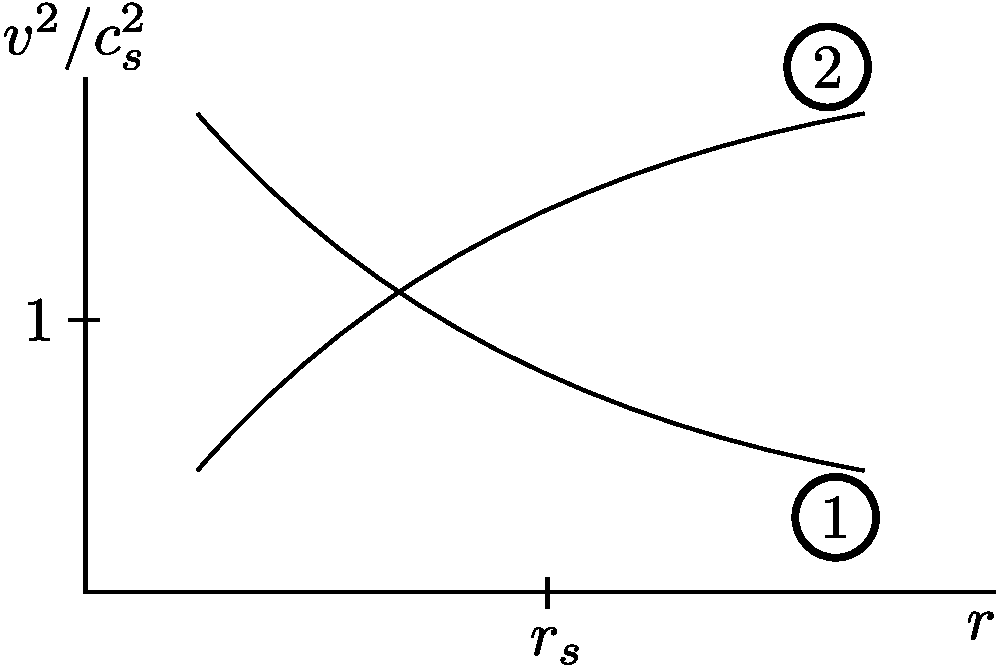
\includegraphics[width = 0.6\textwidth]{figures/sonic_point.pdf}
			\caption{Possible wind solutions from the Parker wind equation. The curve labeled with a circled 1 is the case of accretion, where matter is subsonic past the sonic point and supersonic within. In this case, we expect freefall within the sonic point. The case marked with a circled 2 models a stellar wind, which is inverted.}
			\label{fig:acc:1}			
		\end{figure}
		Now we'll return to the Euler equation and integrate it:
		\begin{equation}
			\label{eq:acc:33} \frac{v^2}{2}+\int \frac{dP}{\rho} - \frac{GM}{r} = \mathrm{const}
		\end{equation}
		Using our polytropic equation of state, we can express the pressure differential as
		\begin{equation}
			\label{eq:acc:34} dP = K\gamma\rho^{\gamma-1}\,d\rho \qquad \Rightarrow \qquad c_s^2 = K\gamma\rho^{\gamma-1} = \frac{\gamma P}{\rho}
		\end{equation}
		where we've utilized the definition of the sound speed to clean things up. Now eq.~\eqref{eq:acc:33} becomes
		\begin{equation}
			\frac{v^2}{2} + \frac{c_s^2}{\gamma-1} - \frac{GM}{\gamma} = \mathrm{const}
		\end{equation}
		This latest form is often referred to as the \textbf{Bernoulli integral}. Now we need to look at the boundary conditions. Specifically, we know that $v^2$ vanishes as $r\to\infty$, so the constant must be 
		\begin{equation}
			\label{eq:acc:35} \mathrm{const} = \frac{\left[c_s(\infty)\right]^2}{\gamma-1}
		\end{equation}
		Additionally, we know that at $r=r_s$, $v = c_s$, so we may simplify to
		\begin{equation}
			\label{eq:acc:36} c_s^2(r_s)\left[\frac{1}{2}+\frac{1}{\gamma-1} - 2 \right] = \frac{cs^2(\infty)}{\gamma-1}
		\end{equation}
		with this solution at hand, we can solve for the sound speed at the sonic point:
		\begin{equation}
			\label{eq:acc:37} c_s(r_s) = c_s(\infty)\left(\frac{2}{5-3\gamma}\right)^{1/2}
		\end{equation}
		Now we can return to our equation for the accretion rate in steady state:
		\begin{equation}
			\label{eq:acc:38} \dot{M} = 4\pi r^2 \rho(-v) = 4\pi r_s^2\rho(r_s)c_s(r_s)
		\end{equation}
		Recall though that $c_s^2\propto \rho^{\gamma-1}$. Then we also know $c_s^2(r_s)/c_s^2(\infty) = \rho(r_s)^{\gamma-1}/\rho(\infty)^{\gamma-1}$. Doing the algebra, this gives the density at the sonic point as
		\begin{equation}
			\label{eq:acc:39} \rho(r_s) = \rho(\infty)\left[\frac{c_s(r_s)}{c_s(\infty)}\right]^{2/(\gamma-1)}
		\end{equation}
		Doing all the substitutions, we get an accretion rate of
		\begin{equation}
			\label{eq:acc:40} 
			\boxed{\dot{M} = \pi G^2 M^2 \frac{\rho(\infty)}{c_s^3(\infty)} \left[ \frac{2}{5-3\gamma}\right ]^{\frac{5-3\gamma}{2(\gamma-1)}}}
		\end{equation}
		This is the main result of Bondi accretion. Note that the term in the brackets is unity for $\gamma = 5/3$ and  $e^{3/2}\approx 4.5$ for $\gamma = 1$. Bondi-Hoyle-Lyttleton accretion is where movement $v(\infty)$ of the body with respect to the gas is $\sqrt{c_s^2(\infty) + v^2(\infty)}$ which gives an accretion rate of
		\begin{equation}
			\label{eq:acc:41} \dot{M} = 4\pi G^2 M^2 \frac{\rho(\infty)}{\left[c_s^2(\infty) + v(\infty)^2\right]^{3/2}} \left[\frac{2}{5-3\gamma}\right]^{\frac{5-3\gamma}{2(\gamma-1)}}
		\end{equation}
		So the overall result is the same as our simple result from earlier, but the prefactors are right now and we can account for motion of the central body within the accreting medium.\\
		
		\n There are, however, some limitations to this theory. There is some fine tuning required depending on the exact boundary conditions. In reality, shocks are expected. Secondly, this theory assumes no heat transport, which is likely not valid on long enough timescales. Thirdly, it is assumed that the accreting material does not radiate, which can become quite important at small distances. Finally, we've assume perfect spherical symmetry and zero angular momentum. Still, though, this basic theory gives us a simple view into the theory of accretion.
		
	% subsection a_more_detailed_calculation (end)
	
	\subsection{Interacting Binaries} % (fold)
	\label{sub:interacting_binaries}
	The majority of high energy stellar-mass phenomena are interacting binaries. These include cataclysmic variables (CVs), Algol systems, W UMa, low mass X-Ray binaries, type Ia Supernovae. If we have two stars of mass $m_1$ and $m_2$, Kepler's third law tells us that their period is given by
	\begin{equation}
		\label{eq:binaries:1} P^2 = \frac{4\pi^2a^3}{G(m_1+m_2)}
	\end{equation}
	where $a$ is the semi-major axis of the orbit. Given enough time, tidal forces will act to circularize the orbit, and if so, $a$ is just the simple separation between the two stars (where $e$, the eccentricity, vanishes). A schematic of such a binary is shown in Figure~\ref{fig:binaries:1}.
	\begin{figure}[h]
		\centering
		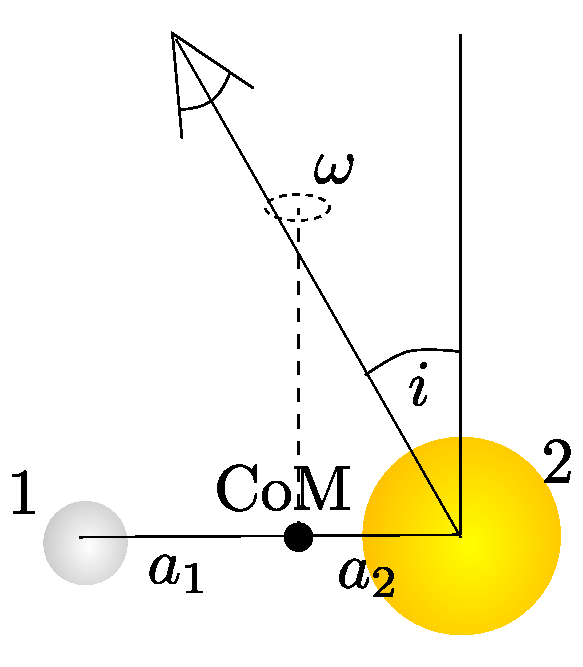
\includegraphics[width = 0.4\textwidth]{figures/interacting_binary.pdf}
		\caption{Schematic of an interacting binary. Stars 1 and 2 orbit about their center of mass as radii $a_1$ and $a_2$, respectively. An observer views this from an angle $i$ with $i=0$ giving a face-on view and $i=90^\circ$ giving an edge-on view.}
		\label{fig:binaries:1}
	\end{figure}
	Regarding the situation shown in Figure~\ref{fig:binaries:1}, we have $a = a_1+a_2$. Kepler's laws mandate $m_1a_1 = m_2a_2$. For convenience, we'll define $M=m_1 + m_2$. Then we can solve for an individual orbital radius of, say, star 1: $a_1/a = m_2/M$. If we can measure (spectroscopically or otherwise) the maximum velocity in the orbit, it will have first been modulated by our viewing angle. Specifically,
	\begin{equation}
		\label{eq:binaries:2} v_1 = v_{1,\mathrm{true}}\sin i = \left(\frac{2\pi}{P}\right)a_1\sin i
	\end{equation}
	for further convenience, we define the \textbf{mass function} via
	\begin{equation}
		\label{eq:binaries:3} f_1(m_1, m_2, i) \equiv \frac{(m_2\sin i)^3}{(m_1+m_2)^2} = \frac{Pv_1^3}{2\pi G}
	\end{equation}
	Define $q = m_1/m_2$ so that $M/m_2 = 1+q$. Then the mass function becomes
	\begin{equation}
		\label{eq:binaries:4} f_1(m_2, i, q) = \frac{m_2(\sin i)^3}{(1+q)^2}
	\end{equation}
	Using this all to solve for the semi-major axis $a$, we get
	\begin{equation}
		\label{eq:binaries:5} \boxed{a = 3\times 10^{11}\ \mathrm{cm}\ \left(\frac{m_2}{M_\odot}\right)^{1/3}(1+q)^{1/3}P^{2/3}}
	\end{equation}
	In general, $f_1 < m_2$ since $(\sin i)^3 \leq 1$ and $(1+q)^{-2} < 1$. If the source is double-lined, then we can measure velocities from both stars. In this case, the mass ratio is simply
	\begin{equation}
		\label{eq:binaries:6} q = \left(\frac{f_2}{f_1}\right)^{1/3}
	\end{equation}
	\subsubsection{Roche Potentials} % (fold)
	\label{ssub:roche_potentials}
		To deal with the equipotential surfaces of such binaries, we first define the angular velocity vector, given by
		\begin{equation}
			\label{eq:binaries:7} \bm{\Omega} = \sqrt{\frac{GM}{a^3}}\,\hat{z}
		\end{equation}
		In the co-rotating frame (where the stars are at rest), the potential has two terms: a gravitational potential and a centrifugal potential. The overall potential is then given by
		\begin{equation}
			\label{eq:binaries:8} \Phi = \Phi_{\mathrm{G}} + \Phi_\Omega = -\frac{Gm_1}{\norm{\mathbf{r}-\mathbf{r}_1}} - \frac{G m_2}{\norm{\mathbf{r}-\mathbf{r}_2}} - \frac{1}{2}(\bm{\Omega}\times \mathbf{r})^2
		\end{equation}
		Where here, the coordinate system has the center of mass of the binary at its origin and, again, it is co-rotating with the binary. Near each star, the potential is like the circular potential of the isolated star, and very far away, the potential is like that from a point source at the center of mass. In the intermediary stages, though, tear-dropped contours form for the equipotential surfaces. An example of such equipotential contours from a binary system is shown in Figure~\ref{fig:binaries:2}.
		\begin{figure}[ht]
			\centering
			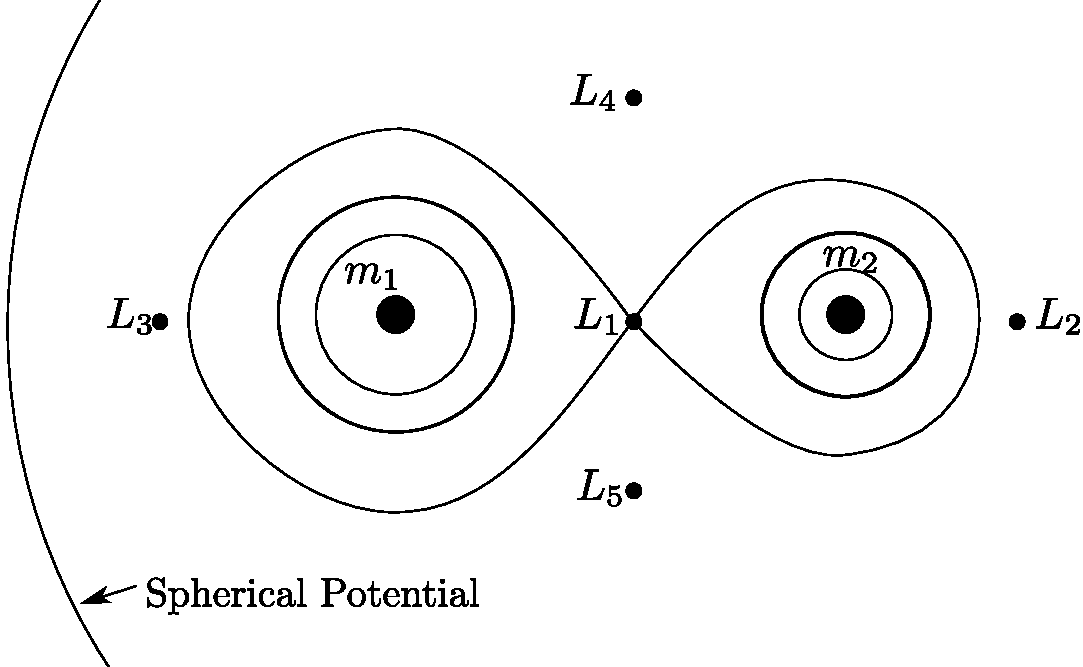
\includegraphics[width=0.6\textwidth]{figures/roche_potentials.pdf}
			\caption{Equipotentials for a binary star system. Those contours closest to the stars resemble spherical potentials about an individual star, and those furthest away resemble contours from a point mass located at the center of mass. The intermediate regime shows distorted shapes resulting from competition between the two stars. Also shown are the Lagrange points as discussed in the text.}
			\label{fig:binaries:2}
		\end{figure}
		There are three main configurations for a binary system with respect to these Roche potentials. A \textbf{detached} binary has both stars situated fully within their Roche lobes (within the potential with $L_1$ in it). A \textbf{semi-detached} binary has one star with a radius that exceeds its Roche lobe. Finally, a \textbf{contact binary} has both stars exceeding their Roche lobe, forming a ``common envelope''. $L_1$, or the inner Lagrange point, is a saddle point. That is, it is a point of quasi-stable equilibrium. It is a maximum in the potential in the $x-$direction and a minimum in the $y$-direction. If expansion proceeds beyond $L_2$ or $L_3$ (which are also saddle points), then mass is lost from the system. $L_4$ and $L_5$ are also local maxima and are thus unstable. These considerations also apply to non-stellar binaries like the Earth and the sun. For instance, WMAP is currently located at $L_2$, and JWST will (hopefully) soon join it. This allows them to be beyond Earth's shadow so they can use solar panels.\\
		
		\n For now, let's assume $m_1>m_2$, and define $R_1$, $R_2$ as the radii of spheres with the radius of the Roche lobe. Remember that $q = m_1/m_2$ (in our definition, it may vary depending on the book you are reading). Furthermore, define $b_1$ and $b_2$ to be the distances from each star to $L_1$. In 1983, Eggleton developed an approximation for the Roche lobe radius:
		\begin{equation}
			\label{eq:binaries:9} \frac{R_2}{a} = \frac{0.49 q^{-2/3}}{0.6 q^{-2/3}+ \ln (1+q^{-1/3})}
		\end{equation}
		For example, if $q=10$, then $R_2/a \approx 0.21$. If we instead wanted to write this explicitly in terms of the masses, then we get
		\begin{equation}
			\label{eq:binaries:10} \frac{R_2}{a} = 0.462\left(\frac{m_2}{m_1+m_2}\right)^{1/3} = 0.462\left(1+q\right)^{-1/3}
		\end{equation}
		but only for the limited range $1.25\leq q \leq 10$. This gives the same result for $q = 10$, though. There is also a semi-analytic approximation for $b_1$, which is the distance from $L_1$ to the primary, $m_1$:
		\begin{equation}
			\label{eq:binaries:11} \frac{b_1}{a} = 0.500 + 0.227\log_{10} q
		\end{equation}
		Now if we consider the case where $m_2$ is overflowing its own Roche lobe, we can calculate the average density inside the Roche lobe by using the orbital period:
		\begin{equation}
			\label{eq:binaries:12} \avg{\rho_2} = \frac{3m_2}{4\pi R_2^3} = \frac{3}{4\pi(0.462)^3a^3}M = \frac{\pi M}{4\pi^2 a^3} = \frac{\pi}{(0.462)^3G P^2}
		\end{equation}
		where we've used Kepler's law to eliminate the semi-major axis. Scaling this result, we get
		\begin{equation}
			\label{eq:binaries:13} \avg{\rho_2} \sim 115 \left(\frac{P}{\mathrm{hr}}\right)^{-2}\ \mathrm{g\ cm^{-3}}
		\end{equation}
		So for binaries with a period of a few hours, those stars with mean densities typical of the lower main sequence with $\avg{\rho}\sim 1 - 100\ \mathrm{g\ cm^{-3}}$ can fill their Roche lobes.
	% subsubsection roche_potentials (end)
	\subsubsection{Mass Transfer and Effects on Orbits} % (fold)
	\label{ssub:mass_transfer_and_effects_on_orbits}
		Before we concluded that for $i,j$ = $1,2$ and $i\neq j$, 
		\begin{equation}
			\label{eq:binaries:14} a_i = \frac{a m_j}{M}
		\end{equation}
		Now the total angular momentum, using the binary's angular frequency, $\omega = 2\pi / P$, is given by
		\begin{equation}
			\label{eq:binaries:15} J = m_1a_1^2 \omega + m_2 a_2^2 \omega + I \omega_1 + I\omega_2
		\end{equation}
		where we are assuming that $I \ll a^2 m$ (the moment of inertia). Dropping those terms and eliminating the orbital radii in favor of masses and the overall semi-major axis, we can get
		\begin{align}
			\label{eq:binaries:16} J &= m_1 a_1^2\omega + m_2 a_2^2\omega\\
			\label{eq:binaries:17} &= \frac{m_2m_1^2a^2}{M^2}\omega + \frac{m_1^2m_2 a^2}{M^2}\omega = \frac{a^2m_1m_2M}{M^2}\omega\\
			\label{eq:binaries:18} &= \frac{m_1m_2}{M}a^2\omega
		\end{align}
		Now if we assume that no mass is lost and no angular momentum is lost (essentially assuming a stream of matter between the two stars with no mass lost along the way), then we have $\dot{m_1} = -\dot{m_2}$ and $\dot{J} = 0$. The effect this has on the period is then
		\begin{equation}
			\label{eq:binaries:19} \frac{\dot{P}}{P} = \frac{3\dot{M}(m_1-m_2)}{m_1m_2}
		\end{equation}
		
	So if the heavier star losses mass, the period decreases, and since $P\propto a^{3/2}$, the orbital separation must also decrease, causing runaway mass transfer (since the Roche lobe shrinks as mass is lost). On the other hand, if the lighter star loss mass, both the period and the orbital separation will increase.\\
	
	\n Often a fraction of the mass lost from one star will be completely lost from the system. This is a common consequence of spherical mass winds. This is called non-conservative mass loss. Let's assume for now that $\dot{m}_1 = 0$ but $\dot{m}_2 \neq 0$. Then the angular momentum loss is
	\begin{equation}
		\label{eq:binaries:20} \dot{J} = \dot{m}_2 a_2^2 \omega
	\end{equation}
	and the orbital separation and period both increase according to
	\begin{equation}
		\label{eq:binaries:21} \frac{\dot{a}}{a} = -\frac{\dot{m}_2}{M} \qquad \Rightarrow \qquad \frac{\dot{P}}{P} = -\frac{2\dot{m_2}}{M}
	\end{equation}
	% subsubsection mass_transfer_and_effects_on_orbits (end)
	% subsection interacting_binaries (end)
	% section accretion_of_astrophysical_plasmas (end)
	\section{White Dwarfs} % (fold)
	\label{sec:white_dwarfs}
	The first discovered white dwarf (WD) was discovered in 1783 by William Herschel. It was discovered in a triple system consisting of 40 Eri A, 40 Eri B, and 40 Eri C. 40 Eri B was the WD what was observed, though it was not well understood at the time. Much later in 1914, Russel (of the Herzprung-Russel diagram) identified the spectrum of 40 Eri B as an A star (taken in 1910). Note that 40 Eri B is not the closest WD, but it is the most easily observed.\\
	
	\n The next WD discovered was Sirius B, which was suspected astrometrically by Bessel as early as 1844. This is because there was an observed departure from linear motion of Sirius A (the really bright star). He wrote in 1844 \begin{quote} The existence of numberless visible stars can prove nothing against the existence of numberless invisible ones. \end{quote} Sirius B was first observed in 1862 by Alvan Graham Clark, and in 1915, Walter Adams obtained a spectrum, declaring that it was both faint and white. Later in 1928, he detected a gravitational redshift in this spectrum, which was actually the first test of GR. He concluded that it was 2000 times denser than platinum.\\
	
	\n In 1927, Eddington mused about Sirius B \begin{quote} The message of Sirius, when it was decoded ran, ``I am composed of material 3,000 times denser than anything you have ever come across; a ton of my material would be a little nugget you could put in a match box.'' What reply can be made of a such a message? The reply most of us made in 1914 was, ``Shut up. Don't talk nonsense.'' \end{quote}
	It wasn't until 1917 that the first isolated WD was discovered van Maanan's star. No new ones were discovered until the 1930's.
	\subsection{Observed Properties of WDs} % (fold)
	\label{sub:observed_properties_of_wds}
	We can break WDs up into classes according to different spectroscopic properties. Each of the classes begin with a ``D'', designating dwarf.
	\begin{itemize}
		\item DA stars show strong hydrogen lines. These constitute about 2/3 of all WDs.
		\item DB stars show strong He I lines, making up about 8\% of all WDs.
		\item DO stars show strong He II lines, making up about 14\% of all WDS.
		\item DC stars show no strong lines and are relatively rare ($\sim 1\%$)
		\item DZ stars show strong metal lines but no carbon. These are also pretty rare.
		\item DQ stars show strong carbon lines, and they make up about 0.1\% of all WDs.
	\end{itemize}
	These spectroscopic classes also show variety in their effective temperatures. DO stars have $T_{\mathrm{eff}}\approx 100,000\ \mathrm{K} - 45,000\ \mathrm{K}$. DB stars are a bit cooler at $30,000\ \mathrm{K} - 12,000\ \mathrm{K}$. DC stars are even cooler, typically less than $12,000\ \mathrm{K}$. DQ stars are typically warmer than 15,000 K.\\
	
	\n The typical mass of a WD is around $0.5-0.6\ M_\odot$ with surface gravities of around $\log g \approx 8.0$. Some of these are variable. ZZ Ceti variables are WDs with $T_{\mathrm{eff}}\approx 12,000\ \mathrm{K}$ with pulsational periods of $P\sim 100 - 1000\ \mathrm{s}$. There are also variable DA stars (DAVs) that exhibit nonradial pulsations that are driven by partial ionization of the hydrogen in their atmospheres. DBV stars act similarly due to partial helium ionization zones at $T_{\mathrm{eff}}\sim 27,000\ \mathrm{K}$. There are also planetary nebula variables (PNNVs) that are present right after the birth of a WD.\\
	
	\n Most WDs are largely composed of carbon and oxygen (C-O WDs), though there are also lower-mass pure He WDs. On the higher end of the mass scale, there are Oxygen-Neon (O-Ne) WDs, but most have hydrogen in their atmospheres. Due to the intense surface gravity, there is thorough surface stratification. That is, there is nearly pure hydrogen on the surface with heavier elements sinking to the lower levels. As a result, DA WDs dominate the population since even a small amount of hydrogen will form a nearly pure layer at the top.
	% subsection observed_properties_of_wds (end)
	\subsection{White Dwarf Structure} % (fold)
	\label{sub:white_dwarf_structure}
		We'll begin by discussing some macroscopic equations governing pressure and density in white dwarfs. Recall that a white dwarf is just the degenerate core of an old star that is so dense that the pressure is due nearly entirely to electron degeneracy pressure. As a result of this, pressure is independent of temperature. Mass conservation tells us that
		\begin{equation}
			\label{eq:wd_struc:1} dm(r) = 4\pi r^2\rho(r)
		\end{equation}
		and hydrostatic balance mandates that
		\begin{equation}
			\label{eq:wd_struc:2} \frac{dP(r)}{dr} = -\frac{Gm(r)\rho(r)}{r^2}
		\end{equation}
		We also want a relationship between the pressure $P$ and the density $\rho$. We'll assume a polytropic equation of state
		\begin{equation}
			\label{eq:wd_struc:3} P = K\rho^\gamma = K \rho^{1+1/n}
		\end{equation}
		where $n$ is the polytropic index. The microscopic properties will give us the polytropic index or $\gamma$ more precisely, but now we'll present a rough derivation as given by Landau.\\
		
		\subsubsection{Equations of State} % (fold)
		\label{ssub:equations_of_state}
		\n Consider a uniform density of fermions (say, electrons). Define the number density as
		\begin{equation}
			\label{eq:wd_struc:4} n = \frac{3N}{4\pi R^3}
		\end{equation}
		where $R$ is the size of the star. The average spacing of the particles is then $\Delta x \approx n^{-1/3}$. Heisenberg's uncertainty principle tells us 
		\begin{equation}
			\label{eq:wd_struc:5} \Delta x \Delta p \sim \hbar \qquad \Rightarrow \qquad \Delta p \sim \frac{\hbar}{\Delta x} \approx \hbar n^{1/3}
		\end{equation}
		Then the total energy, relativistically speaking, is
		\begin{equation}
			\label{eq:wd_struc:6} E^2 = p^2c^2 + m^2c^4
		\end{equation}
		If we assume $pc > mc^2$ (the ultra-relativistic limit), we get an internal energy of (using our momentum relation from above)
		\begin{equation}
			\label{eq:wd_struc:7} E_i \approx pc = \hbar c\left(\frac{3N}{4\pi R^3}\right)^{1/3} = \hbar c\left(\frac{3}{4\pi}\right)^{1/3}\frac{N^{1/3}}{R}
		\end{equation}
		The gravitational energy per fermion of such a uniform density ball would be
		\begin{equation}
			\label{eq:wd_struc:8} E_g = -\frac{3G M}{5 R}
		\end{equation}
		where $M = N m_{\mathrm{particle}}$. The the total energy (the sum of the two) is 
		\begin{equation}
			\label{eq:wd_struc:9} E_{\mathrm{tot}} = E_i + E_G = \frac{1}{R}\left(\hbar c\left(\frac{3}{4\pi}\right)^{1/3}N^{1/3} - \frac{3}{5}G Nm_{\mathrm{particle}}\right)
		\end{equation}
		We find equilibrium when there is no energy gradient, $\partial E/\partial r = 0$ when the right hand side vanishes: 
		\begin{align}
			\label{eq:wd_struc:10} \left(\frac{3}{4\pi}\right)^{1/3}N^{1/3}\hbar c &= \frac{3}{5}GNm_{\mathrm{particle}} \\
			\label{eq:wd_struc:11} N^{2/3} &= \frac{\left(\frac{3}{4\pi}\right)^{1/3}\hbar c}{\frac{3}{5}Gm_{\mathrm{particle}}} \\
			\label{eq:wd_struc:12} N_{\mathrm{critical}} &= \frac{ \left(\frac{3}{4\pi}\right)^{1/2}\left(\hbar c\right)^{3/2}\left(\frac{5}{3}\right)^{3/2} }{ G^{3/2}m_{\mathrm{particle}}^{3/2}}\\
			\label{eq:wd_struc:13} &= \left(\frac{3}{4\pi}\frac{5}{3}\right)^{1/2}\frac{5}{3}\left(\frac{\hbar c}{G m_{\mathrm{particle}}}\right)^{3/2}\\
			\label{eq:wd_struc:14} &= \frac{5\sqrt{5}}{6\sqrt{\pi}}\left(\frac{\hbar c}{Gm_{\mathrm{particle}}}\right)^{3/2}\\
			\label{eq:wd_struc:15} &= 2.3\times 10^{57}\,\mathrm{particles}
		\end{align}
		The corresponding mass is 
		\begin{equation}
			\label{eq:wd_struc:16} M_{\mathrm{max}} = N_{\mathrm{crit}} * m_{\mathrm{particle}} = 1.05 \left(\frac{\hbar c}{G}\right)^{3/2}m_{\mathrm{particle}}^{-2}\sim 1.9\,M_\odot
		\end{equation}
		There have made a lot of approximations here, so now we'll do a more detailed calculation. What's interesting to note, though, is that quantum mechanics, gravitational potential, and electromagnetism were enough to specify the macroscopic mass of the object. If the WD is larger than this, the energy is negative, causing collapse (making this a maximum possible mass attainable by a WD in equilibrium). If it is smaller, then the radius would increase until equilibrium is reached.\\
		
		\n We'll still assume that the average spacing between particles is given by $\Delta x \sim n^{-1/3}$. For degeneracy pressure to be the dominant source of support, we must be in the regime where
		\begin{equation}
			\label{eq:wd_struc:16a} \Delta p c \gg kT
		\end{equation}
		We can effectively treat our white dwarfs as as zero temperature objects then, since kinetic pressure is negligible. Fermi-Dirac statistics give a number density (in phase space) of
		\begin{equation}
			\label{eq:wd_struc:17} \frac{dN}{d^3x\,d^3p} = \frac{g}{\hbar^3}\underbrace{\frac{1}{e^{(E-\mu)/kT}+1}}_{f(E)}
		\end{equation}
		Here, $g$ is a statistical weight that, for electrons is 2 due to the two spin states of the electron. $E$ is the particle energy and $\mu$ is the chemical potential. When quantum effects are unimportant, $f(e)\approx \exp{(\mu-E)/(kT)}$, and the distribution function resembles that of a Maxwell-Boltzmann distribution. At lower temperatures, though, $f(E)$ resembles a step function:
		\begin{equation}
			\label{eq:wd_struc:18} f(E) = \left\{ \begin{array}{ll}
				1 & :E \leq E_{F}\\
				0 & :E > E_F
			\end{array}\right.
		\end{equation}
		where $E_F$ is the Fermi Energy, which is the chemical potential at $T=0$. There is a momentum associated with this energy, given by 
		\begin{equation}
			\label{eq:wd_struc:19} E_F = \left(p_F^2 c^2 + m_e^2c^4\right)^{1/2}.
		\end{equation}
		Now we wish to find the number density, which requires we integrate the distribution function over all momenta:
		\begin{equation}
			\label{eq:wd_struc:20} \frac{N}{d^3x} = n_e = \int_0^\infty dn = \frac{2}{h^3}\int_0^{p_F} 4\pi p^2\,dp
		\end{equation}
		This gives a number density of
		\begin{equation}
			\label{eq:wd_struc:21} n_e = \frac{8\pi}{3h^3}p_F^3
		\end{equation}
		Now solving for the Fermi momentum,
		\begin{equation}
			\label{eq:wd_struc:22} p_F = \left(\frac{3h^3}{8\pi}n_e\right)^{1/3}
		\end{equation}
		Now we can relate the electron number density to the overall mass density via
		\begin{equation}
			\label{eq:wd_struc:23} n_e = \frac{Y_e\rho}{m_{\mathrm{B}}}
		\end{equation}
		where $Y_e$ is the number of electrons per nucleon (typically around a half for a C-O WD due to neutrons). Then the Fermi momentum is
		\begin{equation}
			\label{eq:wd_struc:24} p_F = \left(\frac{3h^3Y_e\rho}{8\pi m_{\mathrm{B}}}\right)^{1/3} \propto \rho^{1/3}
		\end{equation}
		Now we'll look at some limiting regimes. In the nonrelativistic case, we can assume that $p_F\ll m_e c$ and $E_F \approx m_ec^2$. For the relativistic case, $p_F \gg m_e c$ and $E_F \approx pc$. Back to our equation of state, $P=K\rho^\gamma$, we'll find that in the nonrelativistic limit, $\gamma = 5/3$, but in the relativistic regime, $\gamma = 4/3$. We'll now show where these number come from.\\
		
		\n  First, though, we need to revisit the general relation between pressure and energy density, which we'll denote as $\mathcal{E}$. The general relation is
		\begin{equation}
			\label{eq:wd_struc:25} P = (\gamma-1)\mathcal{E}
		\end{equation}
		This $\gamma$ is the same as before, and is the adiabatic $\gamma$, the ratio of specific heats, $\gamma = c_P/c_V$. Now let's use this relation to investigate degeneracy in the nonrelativistic limit. The kinetic energy of a nonrelativistic electron is
		\begin{equation}
			\label{eq:wd_struc:26} E = \frac{1}{2} m_e v^2 = \frac{1}{2} m_e\left(\frac{p^2}{m_e^2}\right) = \frac{p^2}{2m_e}
		\end{equation}
		Assuming a characteristic spacing distance of $\Delta x = a$, or $a = (m_p/\rho)^{1/3}$ this corresponds to
		\begin{equation}
			\label{eq:wd_struc:27}E \approx \frac{\hbar^2}{2m_e a^2}
		\end{equation}
		The energy density then is
		\begin{equation}
			\label{eq:wd_struc:28} \mathcal{E} = E/a^3 \approx \frac{\hbar^2}{2m_ea^5}
		\end{equation}
		Putting this in terms of the density, we get
		\begin{equation}
			\label{eq:wd_struc:29} \mathcal{E} = \frac{\hbar^2}{2m_e}\left(\frac{\rho}{m_{\mathrm{B}}}\right)^{5/3}
		\end{equation}
		Here we've already shown that $\gamma = 5/3$, but we will use the pressure-energy density relation to get
		\begin{equation}
			\label{eq:wd_struc:30} P = \frac{\hbar^2}{3m_e}\left(\frac{\rho}{m_{\mathrm{B}}}\right)^{5/3}
		\end{equation}
		A more careful derivation would give a pressure of
		\begin{equation}
			\label{eq:wd_struc:31} \boxed{P_{\mathrm{non-rel}} = \frac{(3\pi^2)^{2/3}}{5}\frac{\hbar^2}{m_e}Y_e^{5/3}\left( \frac{\rho}{m_e}\right)^{5/3}}
		\end{equation}
		Fantastic. Now let's investigate the relativistic case, where $E \approx pc \approx hc/a$ (via Heisenberg Uncertainty Principle again). Then the energy density is
		\begin{equation}
			\label{eq:wd_struc:32} \mathcal{E} = \frac{E}{a^3} \approx \frac{hc}{a^4} = hc\left(\frac{\rho}{m_p}\right)^{4/3}
		\end{equation}
		So now we see that $\gamma = 4/3$ in the relativistic case. Converting this to pressure in a more detailed calculation gives
		\begin{equation}
			\label{eq:wd_struc:33} \boxed{P_{\mathrm{rel}} = \frac{(3\pi^2)^{1/3}\hbar c Y_e^{4/3}}{4}\left(\frac{\rho}{m_{\mathrm{B}}}\right)^{4/3}}
		\end{equation}
		% subsubsection equations_of_state (end)
		\subsubsection{Mass-Radius Relation for White Dwarfs} % (fold)
		\label{ssub:mass_radius_relation_for_white_dwarfs}
			Linearizing the equation for hydrostatic equilibrium, \eqref{eq:wd_struc:2}, we find
			\begin{equation}
				\label{eq:wd_struc:34} \frac{P}{r}\sim \frac{m(r)\rho}{r^2}\sim r\rho^2
			\end{equation}
			Now mandating that $P\propto \rho^\gamma$, this gives us
			\begin{equation}
				\label{eq:wd_struc:35} \rho^\gamma\sim r^2\rho^2 \qquad \Rightarrow \qquad \rho\sim r^{2/(\gamma-2)}
			\end{equation}
			Now assuming $M\sim \rho r^3$, we find
			\begin{equation}
				\label{eq:wd_struc:36} M\sim r^{\frac{3\gamma - 4}{\gamma - 2}}
			\end{equation}
			So we see that as $\gamma\to 5/3$, we find
			\begin{equation}
				\label{eq:eq:wd_struc:37} R\propto M^{-1/3}
			\end{equation}
			and for the relativistic case ($\gamma = 4/3$), we find that mass is independent of radius!
		% subsubsection mass_radius_relation_for_white_dwarfs (end)
		\subsection{The Chandrasekhar Mass} % (fold)
		\label{sub:the_chandrasekhar_mass}
		\emph{Monday, April 22, 2013}\\
		
		\n We'll only use the first two equations of stellar structure:
		\begin{equation}
			\label{eq:wd_struc:38} \frac{dP}{dr}= -\frac{G M(r)\rho(r)}{r^2} \qquad \frac{dM}{dr} = 4\pi r^2\rho
		\end{equation}
		Now we'll assume a polytropic equation of state, $P=K\rho^\gamma$ to combine these two equations and eliminate $P$ in favor of $\rho$:
		\begin{equation}
			\label{eq:wd_struc:39} \frac{d}{dr}\left(\frac{r^2}{\rho}\frac{dP}{dr}\right) + 4\pi G \rho r^2 = 0
		\end{equation}
		We now change variables to
		\begin{equation}
			\label{eq:wd_struc:40} w = \left(\frac{\rho(r)}{\rho_c}\right)^{1/n}
		\end{equation}
		where $\gamma = 1 + 1/n$. Additionally, we'll express the radial coordinate as $r = az$ where
		\begin{equation}
			\label{eq:wd_struc:41} a = \left[\frac{(n+1)K\rho_c^{1/n - 1}}{4\pi G}\right]^{1/2}
		\end{equation}
		and $z$ is a dimensionless distance. With that witchcraft behind us, eq.~\eqref{eq:wd_struc:39} becomes the \textbf{Lane-Emden Equation}:
		\begin{equation}
			\label{eq:wd_struc:42} \frac{1}{z^2}\left[\frac{d}{dz}\left(z^2\frac{dw}{dz}\right)\right] + w^n = 0.
		\end{equation}
		This equation, in general, cannot be solved analytically, though we can sketch a general set of solutions. Solving the mass equation with this density solution, we get
		\begin{equation}
			\label{eq:wd_struc:43} M = 4\pi \rho_c\int_0^R w^n r^2\,dr = 1.437\,M_\odot\,(2Y_e)^2
		\end{equation}
		where the second expression is in the relativistic limit, i.e., the Chandrasekhar Mass. The radial coordinate is then
		\begin{equation}
			\label{eq:wd_struc:44} R = 3.347\times 10^9\left(\frac{\rho_c}{10^6\ \mathrm{g/cm^3}}\right)^{-1/3}\left(2Y_e\right)^{3/2}\ \mathrm{cm}
		\end{equation}
		for the nonrelativistic case and
		\begin{equation}
			\label{eq:wd_struc:45} R = 1.122\times 10^9\left(\frac{\rho}{10^6\,\mathrm{gm/cm^3}}\right)^{-1/6}\left(2Y_e\right)^{5/6}\ \mathrm{cm}
		\end{equation}
		for the relativistic case. We can express the nonrelativistic mass in terms of the central density or the radius via
		\begin{align}
			M(\rho_c) &= 0.4964\left(\frac{\rho_c}{10^6\,\mathrm{g/cm^3}}\right)6{1/2}\left(2Y_e\right)^{1/2}\,M_\odot\\
			M(R) &= 0.7011 \left(\frac{R}{10^9\,\mathrm{cm}}\right)^{-3}\left(2Y_e\right)^5\,M_\odot
		\end{align}
		% subsection the_chandrasekhar_mass (end)
	% subsection white_dwarf_structure (end)
	\subsection{White Dwarf Cooling} % (fold)
	\label{sub:white_dwarf_cooling}
	Typically a WD isn't just a ball of degenerate matter. There is usually a very thin (by mass) layer of nondegenerate H/He that actually dominates the cooling process of the WD. This is much how the luminosity able to exit a star sets the rate at which fusion occurs at the center. Before we press on, here are some fun facts about WDs. 97\% of stars will end up as WDs. That is, 97\% of stars are less than 8 $M_\odot$. The peak in the WD mass function is around 0.6 $M_\odot$, so we would expect to see a lot of WDs near that mass.\\
	
	\n So the H/He layer is an optically thick insulating layer that keeps the underlying WD hot. The interior is largely isothermal due to the efficiency of heat transport by electrons, and is supported by electron degeneracy. An understanding of the WD cooling process, we must first understand the luminosity of the WD (that is, the rate at which it is losing thermal energy since there is no nuclear energy to power the WD). Radiative diffusion tells us that
	\begin{equation}
		\label{eq:cooling:1} L = -4\pi r^2 \frac{c}{3\kappa\rho} \frac{d}{dr}\left(a T^4\right)
	\end{equation}
	where $a$ is the radiation constant (it's nasty, but built from fundamental constants). $(\kappa \rho)^{-1}$ is the mean free path of photons diffusing through medium, with $\kappa$ being the opacity, with dimension of area per mass (essentially the cross section per unit mass).  Simply carrying through the derivative, we get
	\begin{equation}
		\label{eq:cooling:2} L = -16\pi r^2 \frac{acT^3}{3\kappa\rho}\frac{dT}{dr}
	\end{equation}
	Solving for the temperature gradient, we get
	\begin{equation}
		\label{eq:cooling:3} \frac{dT}{dr} = -\frac{3\kappa \rho}{4acT^3}\frac{L}{4\pi r^2}
	\end{equation}
	If we assume a Kramers' Law dominates the opacity (where $\kappa \propto \rho T^{-3/2}$), we can get a more precise handle on this. For now we'll assume the following parameters
	\begin{align}
		\label{eq:cooling:4} \kappa_0 &= 4.31\times 10^{24} Z(1+X)\,\mathrm{cm^2\,g^{-1}}\\
	\end{align}
	where $\kappa = \kappa_0 \rho T^{-3/2}$. Now, because we know where we're going, we do some bizarre math, where we divide the condition for hydrostatic equilibrium by the temperature gradient to give us $dP/dT$:
	\begin{equation}
		\label{eq:cooing:5} \frac{dP}{dr} = -\frac{GM(r)\rho(r)}{r^2} \qquad \Rightarrow \qquad \frac{dP}{dT} = \frac{16\pi ac GM T^{-6.5}}{3\kappa_0 L \rho}
	\end{equation}
	where we've approximated $M(r)\approx M$ in the outermost layers of the WD. We can eliminate $\rho$ by using the relation between pressure, density, and temperature. We will assume an ideal gas equation of state to do so, meaning that $\rho = P\mu m_{\mathrm{B}}/(kT)$. This gives us
	\begin{equation}
		\label{eq:cooling:6} P\,dP = \frac{16\pi ac G M k}{3 \kappa_0 L \mu m_{\mathrm{B}}} T^{7.5}\,dT
	\end{equation}
	Integrating this from the surface inwards, we get
	\begin{equation}
		\label{eq:cooling:7} \int_0^P p\,dp = \mathcal{G} \int_0^T \tau^{7.5}\,d\tau
	\end{equation}
	where we're assuming a $P=T=0$ boundary condition at the ``surface'', and $\mathcal{G}$ holds all those stupid constants. The resulting equation relating density to temperature is
	\begin{equation}
		\label{eq:cooling:8} \boxed{\rho = \left(\frac{64 \pi a c G M \mu m_{\mathrm{B}}}{51 \kappa_0 L k}\right) T^{13/4}}
	\end{equation}
	Gross, right? Now at some point, the density is high enough so that the matter becomes degenerate and these approximations fail. At this point, $T_{*}\sim T_c$ due to the isothermal nature of degenerate material. Additionally,
	\begin{equation}
		\label{eq:cooling:9} \frac{\rho_* k T_*}{\mu_e m_{\mathrm{B}}} = 1.0\times 10^{13} \left(\frac{\rho_*}{\mu_e}\right)^{5/3}
	\end{equation}
	where $\mu_e = 1/Y_e$. This is essentially stating that the pressure due to an ideal gas (the LHS) is equation to that from degenerate electrons (the RHS). We can solve for this critical density at which degeneracy takes over to find
	\begin{equation}
		\label{eq:cooling:10} \rho_* \approx 48\,\mathrm{g\,cm^{-3}}\left(\frac{\mu_e}{2}\right)\left(\frac{T_*}{10^6\ \mathrm{K}}\right)^{3/2}
	\end{equation}
	Now solving for the luminosity  as a function of the core temperature, we find
	\begin{equation}
		\label{eq:cooling:11} L = 1.43\times 10^{-7}\,L_\odot\,\frac{\mu}{\mu_e}\frac{1}{Z(1+X)} \left(\frac{M}{M_\odot}\right)\left(\frac{T_c}{10^6\,\mathrm{K}}\right)
	\end{equation}
	Or more succinctly, $ L = CMT_c^{7/2}$ where $CM_\odot = 2\times 10^6$ erg/s. Now we might ask what the characteristic cooling time is. What is the timescale on which the temperature will change significantly? If we have the luminosity, we should also figure out what the thermal energy of the WD is, since that is what is initially being radiated away, though crystallization energy losses eventually become important. Assuming ideal gas internal energy, the thermal energy is approximately
	\begin{equation}
		\label{eq:cooling:12} E_{\mathrm{thermal}} = \frac{3}{2} N k T_c = \frac{3}{2} \left[\frac{ M }{ 23 m_{\mathrm{B}}}\right]k T_c
	\end{equation}
	assuming pure carbon-12 in the core. A typical energy at birth would be about $E_{\mathrm{birth}}\sim 10^{58}\ \mathrm{erg}$for a 0.4 $M_\odot$ WD at $T_c\sim 10^8\ \mathrm{K}$. Assuming that the luminosity is the time rate of change of the thermal energy, or
	\begin{equation}
		\label{eq:cooling:13} -\frac{dE}{dt} = L \qquad \Rightarrow \qquad \frac{3}{2} \frac{k m}{A m_{\mathrm{B}}} \frac{dT_c}{dt} = CM T_c^{7/2}
	\end{equation}
	(where $A$ is the average mass number of core material.) Integrating, we find
	\begin{equation}
		\label{eq:cooling:14} \frac{3}{5} \frac{k}{A m_{\mathrm{B}}}\left(T^{-5/2} - T_0^{5/2}\right) = C (t-t_0)
	\end{equation}
	For some constant $C$. If we assume that at early times, $T_0 \gg T$ and defining $t_0=0$, we get
	\begin{equation}
		\label{eq:cooling:15} \frac{3 k T^{-5/2}}{5 A m_{\mathrm{B}}} \approx Ct
	\end{equation}
	Solving for this time, we get
	\begin{equation}
		\label{eq:cooling:16} t = \frac{3k M T}{5 A m_{\mathrm{B}} L}
	\end{equation}
	Parameterizing this result, we have
	\begin{equation}
		\label{eq:cooling:17} t \approx 10^8\ \mathrm{yrs}\ A^{-1}\left(\frac{M/M_\odot}{L/L_\odot}\right)^{5/7}
	\end{equation}
	
	% subsection white_dwarf_cooling (end)
	\subsection{Cataclysmic Varaiables} % (fold)
	\label{sub:cataclysmic_varaiables}
	\emph{Wednesday, April 24, 2013}\\
	
	\n A \textbf{cataclysmic variable} (CV) is a binary system typically consisting of either a main sequence (MS) or red giant (RG) and a white dwarf (WD) with the MS/RG star overflowing its Roche lobe (RLOF for Roche Lobe OverFlow) and donating matter to the WD. These binaries typically have periods of 80 minutes to several hours. CVs give off radiation from several sources
	\begin{itemize}
		\item Secondary (MS/RG)
		\item Accretion Disk
		\item Bright spot where accreted material hits disk
		\item WD surface
	\end{itemize}
	Different sources are relevant for different types of CVs, which we'll now summarize.
	
	\subsubsection{Classical Novae} % (fold)
	\label{ssub:classical_novae}
	A classical nova (CN) has a rapid rebrightening of 6 to 19 magnitudes in the optical. We only see one of these outbursts (as opposed to a recurrent nova, which we'll discuss later). Our current understanding of what causes these events is the accumulation of hydrogen on a WD, followed by ignition at the base in degenerate conditions. As the hydrogen burns to helium, the temperature grows at constant pressure (due to the degenerate nature of the material, which doesn't care about the temperature). This causes a runaway which results in removing a lot of the hydrogen-rich material. We expect there to be about 30 of these each year in the Milky Way, though we may not see most of them due to dust extinction.\\
	
	\n During an outburst, CNe reachs the Eddington luminosity, at which point the hydrogen rich material is blown off of the surface with wind velocities on the order of 1000 km/s over a timescale of days to weeks. Recall that the Eddington luminosity
	\begin{equation}
		\label{eq:cv:1} L_{\mathrm{Edd}} \sim 1.34\times 10^{38}\ \left(\frac{M}{M_\odot}\right)\ \mathrm{erg\ s^{-1}} \sim 10^{38}\ \mathrm{erg\ s^{-1}}
	\end{equation}
	Then the total radiated energy is approximately
	\begin{equation}
		\label{eq:cv:2} E_{\mathrm{tot}} = L_{\mathrm{Edd}}\Delta t \sim 10^{45}\ \mathrm{erg}
	\end{equation}
	which corresponds to approximately $10^{-7}\ M_\odot$ of hydrogen burned to helium. At an accretion rate of $\dot{M}\sim 10^{-10}\ M_\odot/\mathrm{yr}$, we would expect these to go off about every 1000 years (so not recurrent on our timescales).\\
	
	% subsubsection classical_novae (end)
	\subsubsection{Recurrent Novae} % (fold)
	\label{ssub:recurrent_novae}
		Recurrent novae are very similar to classical novae, but they reoccur on timescales of decades. These explosions are less violent, causing less mass loss. This is likely because the ignition takes place when the material is still nondegenerate.
	% subsubsection recurrent_novae (end)
	\subsubsection{Dwarf Novae} % (fold)
	\label{ssub:dwarf_novae}
	A dwarf novae is a rebrightening of around 2 to 5 magnitudes, thought to be linked with accretion. An instability in the accretion disk causes a short increase in the accretion rate, resulting in an increase in brightness. These events can occur with recurrence times on the order of days to weeks or longer. A dwarf nova (while active) has a luminosity of approximately $L\sim 10^{34}\ \mathrm{erg\ s^{-1}}$.\\
	
	% subsubsection dwarf_novae (end)
	\subsubsection{Magnetic CVs} % (fold)
	\label{ssub:magnetic_cvs}
	Magnetic CVs are accreting WDs with very strong magnetic fields ($\sim 10^7\ \mathrm{Gauss}$) where the accreted matter is funneled to the magnetic poles. They have a high state and a low state of emission. A classic example of these is T Cor Bor, which consists of a giant and a magnetized WD, which exhibits recurrent high states.
	% subsubsection magnetic_cvs (end)
	\subsubsection{General Considerations} % (fold)
	\label{ssub:general_considerations}
	\n Let's look at the orbital dynamics of such system. Kepler's Third Law (with some sensible scaling) is
	\begin{equation}
		\label{eq:cv:3} a = \left(3.5\times 10^{10}\ \mathrm{cm}\right)\left(\frac{P}{\mathrm{hr}}\right)^{2/3} \left(\frac{M}{M_\odot}\right)^{1/3}
	\end{equation}
	For reference, a solar radius is $R_\odot = 7\times 10^{10}\ \mathrm{cm}$ and for a WD, $R_{\mathrm{WD}}\sim 5\times 10^{8}\ \mathrm{cm}$, so these are very tight binaries!\\
	
	\n At the innermost region of an accretion disk, there is a boundary layer where the material first ``enters'' the WD. From the virial theorem, we can assume that the material passing through this boundary layer has half of its energy radiated away and half enters the star as heat. The accretion luminosity is
	\begin{equation}
		\label{eq:cv:4} L = \frac{GM_{\mathrm{WD}}\dot{M}}{R_{\mathrm{WD}}}
	\end{equation}	
	Half of this is radiated away and appears as radiation from the disk
	\begin{equation}
		\label{eq:cv:5} L_{\mathrm{disk}} = L_{\mathrm{BL}} \sim \frac{GM_{\mathrm{WD}}\dot{M}}{2 R_{\mathrm{WD}}}
	\end{equation}
	If we assume some characteristic values of $R_{\mathrm{WD}}=6\times 10^{8}\ \mathrm{cm}$, $M_{\mathrm{WD}}= M_\odot$, and $\dot{M} = 1.6\times 10^{-10}\ M_\odot\ \mathrm{yr}$, we get an accretion luminosity of $L\sim 10^{33}\ \mathrm{erg\ s^{-1}}$. Assuming a perfect blackbody is generating this luminosity (and that the energy is radiating away from both sides of the disk), we can use the Stefan-Boltzmann law to solve for a characteristic temperature:
	\begin{equation}
		\label{eq:cv:6} 2\pi R_{\mathrm{disk}}^2\sigma T_{\mathrm{out}}^4 \approx \frac{GM_{\mathrm{WD}}\dot{M}}{ R_{\mathrm{WD}} }
	\end{equation}
	Using $R_{\mathrm{disk}}=4\times 10^{10}\ \mathrm{cm}$ and our previous assumptions, we get $T_{\mathrm{disk}}\approx 2\times 10^3\ \mathrm{K}$.\\
	
	\n Now, if all of the radiation comes from the inner radius, the above analysis must be adjusted to reflect $R_{\mathrm{disk}}\to R_{\mathrm{WD}}$. This results in a temperature of $T_{\mathrm{max}}\approx 5\times 10^4\ \mathrm{K}$. So the range of temperatures is $10^3-10^5\ \mathrm{K}$ , and it would radiate primarily in the visible to ultraviolet. In reality, the bounding layer can be smaller than $2\pi R_{\mathrm{WD}}^2$ if it is an annulus which causes the temperature to go even higher into the extreme UV or soft X-Rays.\\
	
	\n In magnetic WDs, the flux is channeled to a small polar cap $\sim 10\ \mathrm{km}$ with ree-fall velocities, so the temperatures can be as high as $T\sim 10^8\ \mathrm{K}$ ($\sim$10 keV). There may also be circularly polarized radiation at cyclotron frequencies of
	\begin{equation}
		\label{eq:cv:7} \nu = \frac{eB}{m_e c} = 2.8\times 10^{13}\ \mathrm{hz}\ \left(\frac{B}{10^7\ \mathrm{G}}\right)
	\end{equation}
	which is in the near IR. This radiation would be absorbed by the WD and re-radiated in the EUV to optical ranges. A spectrum from a CV will have low frequency components from a companion red star, medium frequency components from an accretion disk, and/or high frequency components from the boundary layer where the material meets the WD.
	% subsubsection general_considerations (end)
	% subsection cataclysmic_varaiables (end)
	% section white_dwarfs (end)
	\section{Neutron Stars} % (fold)
	\label{sec:neutron_stars}
	Neutron stars were first discovered in 1967 by Jocelyn Bell and Hewish (Hewish later got a Nobel prize). They discovered pulsars through radio observations, originally thinking they might be aliens. After discovering several of these LGMs (Little Green Men), they concluded that they were not, in fact, aliens, but some astrophysical object.\\
	
	\n When a WD's mass exceeds the Chandrasekhar mass, it will begin to collapse as the pressure from degenerate electrons can no longer halt the gravitational force. This can also occur in a degenerate core of a massive store (like an iron core). Note that this is \emph{not} what causes a Type Ia supernova. Those start when a C-O WD \emph{approaches} $M_{\mathrm{Ch}}$, triggering explosive carbon burning. \emph{Exceeding} $M_{\mathrm{Ch}}$ results in collapse to a neutron star.\\
	
	\n At some point, the electrons' Fermi energy,
	\begin{equation}
		\label{eq:neutron:1} E_{\mathrm{F}}(e^-) = \sqrt{(p_{\mathrm{F}}c)^2 + (m_ec^2)}
	\end{equation}
	exceeds
	\begin{equation}
		\label{eq:neutron:2} (m_n - m_p)c^2 = 1.29\ \mathrm{MeV}
	\end{equation}
	This happens at a density of $\rho_0 = 1.2\times 10^7\ \mathrm{g\ cm^{-3}}$. At higher densities, it becomes energetically favorable for electrons to inverse beta decay:
	\begin{equation}
		\label{eq:neutron:3} e^- + p \to n + \nu_e
	\end{equation}
	This leads to more and more neutrons and, ultimately, a neutron star.\\
	
	\n More realistically, the WD contains nuclei (C and O, or O and Ne, etc.) and not free neutrons, protons, and electrons. Electrons capture onto nuclei to form increasingly neutron-rich nuclei. At a density of $\rho \approx 4.3\times 10^{11}\ \mathrm{g\ cm^{-3}}$ neutrons begin to bleed from nuclei. This process is called ``neutron drip'' which ``softens'' the equation of state. The star continues to collapse until $\rho>10^{14}\ \mathrm{g\ cm^{-3}}$, at which point neutron degeneracy pressure becomes strong enough to halt further compression. Note that normal nuclear matter (that is, nuclei) has a density of $\rho_{\mathrm{nuc}}\approx 2.8\times 10^{14}\ \mathrm{g\ cm^{-3}}$. The equation of state at these high densities is highly uncertain and is sensitive nuclear theory.\\
	
	\n The actual structure of a neutron star is a bit of a mystery, but if it is indeed just bare neutrons (it probably isn't), we can get some intuition from nuclear physics. The actual equation of state in a neutron star is highly uncertain. The radius of a nucleus is approximately given by $R_{\mathrm{nuc}}\sim A^{1/3}$ where $A$ is the mass number. The ``radius'' of a nucleon is $r_0 = 1.25\ \mathrm{fm}=1.25\times 10^{-13}\ \mathrm{cm}$, so the density of such nuclear matter is $\rho_{\mathrm{nuc}} = 3 A^{1/3}m_n/(4\pi R_{\mathrm{nuc}}^3)$.
	\subsection{Relativistic Caveats} % (fold)
	\label{sub:relativistic_caveats}
	 The Schwarzschild radius for a $1.4\ M_\odot$ black hole is about 3 km, so the general relativistic corrections are important in neutron stars, on the order of $20\%$. The Schwarzschild radius is
	\begin{equation}
		\label{eq:relativistic:1} R_{\mathrm{Sch}} = \frac{GM}{c^2}
	\end{equation}
	so we expect to see gravitational redshifts of 
	\begin{equation}
		\label{eq:relativistic:2} \frac{GM}{c^2R} \sim \frac{\Delta \lambda}{\lambda} = z \approx 0.2
	\end{equation}
	Such deviations in spectra are indeed observed in known neutron stars. As a result of general relativistic corrections, the standard equation of hydrostatic equilibrium is no longer valid. Instead, we must use the TOlman-Oppenheimer-Vokoff (TOV) equation, which is derived from assuming a spherically symmetric metric (and nearly nothing else!) in general relativity.\\
	
	\n At masses above $M=M_\odot$, (and densities above nuclear densities), the equation of state breaks down. This adds an additional uncertainty to the mass-radius relation since things like nucleon-nucleon repulsion might soften the equation of state, but if new particles are created at high densities, this too might soften the equation of state. A softer equation of state means that there is a lower maximum mass. The mass limit for neutron stars is highly uncertain. We typically think it is somewhere around 2 $M_\odot$ to $3.2\ M_\odot$. Most neutron star masses are clustered around $1.4\ M_\odot$.
	% subsection relativistic_caveats (end)
	\subsection{Neutron Star Structure} % (fold)
	\label{sub:neutron_star_structure}
	The general picture of a neutron star consists of an atmosphere, an outer crust, an inner crust, and outer core, and an inner core. The outer parts are fairly well understood, but as we move inwards, less and less is known. From the atmosphere through both crusts, it is estimate that about 1\% of the mass is accounted for. The rest is in the core material.
	\paragraph{Atmosphere} % (fold)
	\label{par:atmosphere}
	At a temperatures of about $3\times 10^6\ \mathrm{K}$, this is about 10 cm thick, and for temperatures of about $3\times 10^5\ \mathrm{K}$, about 10 mm thick. We don't really understand the atmosphere with magnetic fields with $B>10^{11}\ \mathrm{G}$ or temperatures $T<10^6\ \mathrm{K}$. Typically the density follows $\rho\leq 10^6\ \mathrm{g\ cm^{-3}}$ and the total mass in the atmosphere is negligible and comprised largely of ${}^{56}\mathrm{Fe}$. This atmosphere shapes the emerging spectrum and contains a plasma layer that is highly ionized. The atomic energy levels are significantly distorted by the magnetic fields. For $B\sim 10^{12}\ \mathrm{G}$, atoms are shaped like needles. These weirdly-shaped atoms are the reasons why the atomic levels are distorted.
	% paragraph atmosphere (end)
	\paragraph{Outer Crust} % (fold)
	\label{par:outer_crust}
	The outer crust is basically white dwarf material.  The densities range from the atmospheric density up to $\rho \sim 14\times 10^{11}\ \mathrm{g\ cm^{-3}}$. It is on the order of 100 m thick, and at the top, the dominant nucleus if ${}^{56}\mathrm{Fe}$. There are non-degenerate to degenerate electrons present, and at high depths, the material is solid. Electron capture onto nuclei occurs, causing neutron drip at the bottom of the crust which forms a neutron gas with density $\rho\sim 4\times 10^{11}\ \mathrm{g\ cm^{-3}}$.
	% paragraph outer_crust (end)
	\paragraph{Inner Crust} % (fold)
	\label{par:inner_crust}
	The inner crust is approximately 1 km thick. The densities range from $\rho_{\mathrm{drip}}$ to $0.5\rho_{\mathrm{nuc}}$, where you may recall that $\rho_{\mathrm{nuc}}\approx 2.8\times 10^{14}\ \mathrm{g\ cm^{-3}}$. The matter consists of electrons, free neutrons, and neutron-rich nuclei. The preferred nucle become more and more neutron as the density is increased. The nucleon number reaches several, unlike on Earth. These nuclei are just no possible in pretty much any other place in the universe. However, the nuclei number goes to zero at the core boundary as the nuclei get distorted into strange shapes. This gives rise to the colorful terminology of nuclear pasta. Spherical nuclei are called meatballs, long thin nuclei are spaghetti, and nuclear slabs are called lasagna. There are also lattice inverts, which are voids embedded in nuclear matter, called swiss chese. Finally, there are touching nucleons touching, forming a uniform nuclear fluid (the ``sauce''). It may be that this nucleon fluid is a superfluid at low temperatures, which would result in a vanishing viscosity in the fluid. The equation of state is relatively well-known for the crust.
	% paragraph inner_crust (end)
	\paragraph{Outer Core} % (fold)
	\label{par:outer_core}
	Here the density ranges from $0.5\rho_{\mathrm{nuc}}<\rho < 2\rho_{\mathrm{nuc}}$, and the neutron to proton ratio is approximately $n/p>20$. Nuclei essentially cease to exist and the matter transitions to a neutron-proton fluid with negatively charged stuff. In this regime, nucleon-nucleon repulsion becomes important, and the neutrons become superfluid. Along with the inner core, this contains 99\% of the mass.
	% paragraph outer_core (end)
	\paragraph{Inner Core} % (fold)
	\label{par:inner_core}
	Here the densities are greater than $\rho\geq 2\rho_{\mathrm{nuc}}$ and possibly as high as $10-15\rho_{\mathrm{nuc}}$. The equation of state is unknown. It could consist of quark matter, hyperons (baryons that contain strange quarks), pions, or kaons\ldots we don't really know.
	% paragraph inner_core (end)
	% subsection neutron_star_structure (end)
	\subsection{Superfluidity} % (fold)
	\label{sub:superfluidity}
	At temperatures less than some critical temperature $T_c$, we get superfluidity, which is a phenomenon that does not affect the equation of state. It does, however, affect heat capacity and thus neutron star cooling. Protons become superconducting and the magnetic field becomes quantized into flux tubes. The magnetic field freezes in the crust, causing co-rotation of the crust and core (making essentially solid-body rotation).
	% subsection superfluidity (end)
	% section neutron_stars (end)
\section{X-Ray Binaries} % (fold)
\label{sec:x_ray_binaries}
	An \textbf{X-Ray Binary} (XRB) is a binary consisting of a neutron star or black hole with some other companion. Their radiation peaks at $0.1-100\ \mathrm{keV}$. The radiative efficiencies of their accretion power are
	\begin{equation}
		\label{eq:x_ray_binary:1} \eta-{\mathrm{NS}} = \frac{GM}{Rc^2} \approx 0.1
	\end{equation}
	for a neutron star and about $0.4$ for a black hole. This means that 10 and 40 percent of the rest energy of accreted material is radiated away upon accretion. This means that the energy generation rate per unit mass is approxmately
	\begin{equation}
		\label{eq:x_ray_binary:2} \epsilon_{\mathrm{NS}}\sim 10^{20}\ \mathrm{erg\ g^{-1}}
	\end{equation}
	Compare this to hydrogen fusion, which has only $\epsilon_{\mathrm{CNO}}=6\times 10^{18}\ \mathrm{erg\ g^{-1}}\approx 0.007c^2$. The luminosity of X-Ray binaries is usually Eddington-limited, with $L=L_{\mathrm{Edd}}sim 10^{38}\ \mathrm{erg\ s^{-1}}$ and an accretion rate of $\dot{M}\sim 10^{-8}\ M_\odot\ \mathrm{yr^{-1}}$. Comparing this luminosity to a typical radius of $R\sim 10^6\ \mathrm{cm}$ gives a blackbody temperature of $T\approx \times 10^{7}\ \mathrm{K}$. So, these are \emph{hot} surfaces. This corresponds to a frequency of $\nu=1.2\times 10^{18}\ \mathrm{Hz}$, a wavelength of $\lambda = 25\ \textrm{\AA}$, or a photon energy of $h\nu = 5\ \mathrm{keV}$.\\
	
	\n We encounter XRBs in two main flavors. The first is a \textbf{Low Mass X-Ray Binary} (LMXRB), which consists of a neutron star and a main sequence star that is undergoing Roche lobe overflow onto its compact companion. A prime example of a LMXRB is the 1972 discovery of Her X-1 with its 1.24 second period (which is the rotation period of the neutron star) and a secondary 1.7 day period (which is the period of the orbit). Additionally, we observe \textbf{High Mass X-Ray Binaries} (HMXRB), which have a neutron star and an OBstar that is emitting matter via a wind, such as Cen X-3 (1971), which has a 2.1 day period.\\
	
	\n The maximum temperature will occur when free falling matter hits the neutron star surface at $v_{\mathrm{ff}}\sim 0.1c$. This gives a temperature of
	\begin{equation}
		\label{xrb:3} \frac{1}{2}m_p v_{\mathrm{ff}}^2 = \frac{3}{2}k T_{\mathrm{eff}} \qquad \Rightarrow \qquad T_{\mathrm{eff}} = 3.6\times 10^{12} \left(\frac{v_{\mathrm{ff}}}{c}\right)\ \mathrm{K}
	\end{equation}
	Where the free fall velocity is
	\begin{equation}
		\label{eq:xrb:4} v_{\mathrm{ff}} = \left(\frac{2GM}{r}\right)^{1/2}
	\end{equation}
	Usually we see $T\sim T_{\mathrm{Blackbody}}$ rather than $T_{\mathrm{ff}}$.\\
	
	\subsection{Magnetic Inflows} % (fold)
	\label{sub:magnetic_inflows}
	\n The intense magnetization of neutron stars (e.g.\ $B\sim 10^{12}\ \mathrm{G}$) can also disrupt the usual accretion flow at the magnetic (or Alfv\'en) radius, $R_{\mathrm{M}}$, at which the magnetic field pressure equals the ram pressure of freefall. Algebraic, this condition is denoted by
	\begin{equation}
		\label{eq:xrb:5} \rho v_{\mathrm{ff}}^2 = \frac{B^2}{8\pi}
	\end{equation}
	where $B^2$ has energies of energy per volume (i.e., pressure). If we have spherical symmetry, the accretion rate is
	\begin{equation}
		\label{eq:xrb:6} \dot{M} = 4\pi r^2\rho v_{\mathrm{ff}}
	\end{equation}
	and the magnetic field is
	\begin{equation}
		\label{eq:xrb:7} \norm{B} = \frac{\mu}{r^3}\sim 10^{12}\ \mathrm{G} \ \textrm{ where $r=R_{\mathrm{NS}}$}
	\end{equation}
	where $\mu$ is the magnetic dipole moment of the neutron star. We can solve eq.~\eqref{eq:xrb:6} for the density at $r = R_\mathrm{M}$ to get
	\begin{equation}
		\label{eq:xrb:8} \rho = \frac{\dot{M}}{4\pi R_{\mathrm{M}}v_{\mathrm{ff}}}
	\end{equation}
	where now
	\begin{equation}
		\label{eq:xrb:9} v_{\mathrm{ff}} = \left(\frac{2GM}{R_{\mathrm{M}}}\right)^{1/2}
	\end{equation}
	Then the condition to find $R_{\mathrm{M}}$, eq.~\eqref{eq:xrb:5}, becomes
	\begin{equation}
		\label{eq:xrb:10} \frac{(2GM)^{1/2}\dot{M}}{4\pi R_{\mathrm{M}}^{5/2}} = \frac{\mu^2}{8\pi R_{\mathrm{M}}^6}
	\end{equation}
	Solving this for $R_{\mathrm{M}}$ gives us
	\begin{equation}
		\label{eq:xrb:11} R_{\mathrm{M}}=(8G)^{-1/7}\mu^{4/7}\dot{M}^{-2/7}M^{-1/7}
	\end{equation}
	Now if we use the XRB's luminosity as $L_X = GM\dot{M}/R$ to parameterize $R$, we get
	\begin{multline}
		\label{eq:xrb:12} R_{\mathrm{M}} = 2.9\times 10^8\ \mathrm{cm}\ \left(\frac{M}{M_\odot}\right)^{-1/7} \left(\frac{R}{10^6\ \mathrm{cm}}\right)^{-2/7}\left(\frac{L_X}{10^{37}\ \mathrm{erg\ s^{-1}}}\right)^{-2/7}\\
		\times \left(\frac{\mu}{10^{30}\ \mathrm{G\ cm^{-3}}}\right)^{4/7} \approx 3\times 10^8\ \mathrm{cm}
	\end{multline}
	This radius is several hundred neutron star radii, so this magnetic distortion is an observable effect. The picture is then some accretion disk that has some inner radius where matter is then channeled along field lines to the polar caps. Such a configuration is shown in Figure~\ref{fig:xrb:1}.
	\begin{figure}[ht]
		\centering
		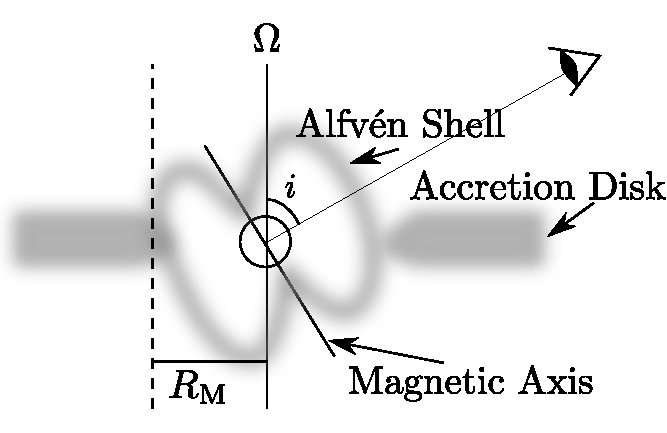
\includegraphics[width = 0.6 \textwidth]{figures/alfven_shell.pdf}
		\caption{A sketch of magnetically distorted accretion. Material outside $R_{\mathrm{M}}$ forms a normal accretion disk, but within $R_{\mathrm{M}}$, it is channeled along magnetic field lines to the magnetic polar caps, which may or may not be along the same axis as the rotation axis.}
		\label{fig:xrb:1}
	\end{figure}
	The magnetic channeling of material causes a relatively small magnetic cap area to be heated by the infalling plasma. The incoming matter int his region will be revolving about the magnetic fields at the cyclotron frequency, which for electrons is 
	\begin{equation}
		\label{eq:xrb:13} E_{\mathrm{cyc}} = h\nu_e = 11.6\left(\frac{B}{10^{12}\ \mathrm{G}}\right)\ \mathrm{keV}
	\end{equation}
	and for protons
	\begin{equation}
		\label{eq:xrb:14} E_{\mathrm{cyc}} = h\nu_p = 6.3\left(\frac{B}{10^{15}\ \mathrm{G}}\right)\ \mathrm{keV}
	\end{equation}
	So the energies of these particles are quantized for motion perpendicular to the field. These quantized levels are called Landau levels and are given by
	\begin{equation}
		\label{eq:xrb:15} h\nu = (n+\frac{1}{2} + s)E_{\mathrm{cyc}}
	\end{equation}
	where $n$ is the quantum number and $s=\pm 1/2$ is the spin of the particle. Thus there will be increased Compton scattering at these quantized energies, which was seen in M Her X-1 in the 1970s in the absorption spectrum. The relativistic redshift is important here, too, since $h\nu_{\mathrm{obs}} = h\nu_{\mathrm{cyc}}/(1+z)$.\\
	
	\n We already stated that the magnetic field may be misaligned with the rotation axis. This misalignment gives rise to X-Ray pulsations. These, too, are observed. For example, a period of 0.7145 s is observed in SMC X-1 and 0.069 in A05388-66 (cool name, huh?).\\
	
	\n The accreted material can also act to spin up the neutron star by taking angular momentum from the disk and depositing it in the neutron star. For example, millisecond pulsars are found in binaries and are thought to have been spun-up over the course of their accretion lives.
	% subsection magnetic_inflows (end)
	\subsection{Pulsar Spindown} % (fold)
	\label{sub:pulsar_spindown}
	If a relatively slowly spinning neutron star can be spun up by accreting material, a rapidly-rotating neutron star should be able to spun \emph{down} by the accreted material. For example, the Crab pulsar, which is a remnant of SN 1054 has a period of $P=33\ \mathrm{ms}$, but it is slowing down at $dP/dt\sim 1\ \mathrm{ms}/(100\ \mathrm{yrs})$.\\
	
	\n If we approximate a neutron star as a uniform sphere, then the moment of inertia is
	\begin{equation}
		\label{eq:spindown:1} I = \frac{2}{5}M R^2 = 2.5\times 10^{45}\ \left(\frac{M}{1.4\ M_\odot}\right) \left(\frac{R}{1.5\times 10^6\ \mathrm{cm}}\right)^{2}\ \mathrm{g\ cm^2}
	\end{equation}
	The crab pulsar spins down at a rate
	\begin{equation}
		\label{eq:spindown:2} \frac{d\omega}{dt} = -2.4\times 10^{-9}\ \mathrm{s^{-2}}
	\end{equation}
	where $\omega$ is the angular velocity. This implies a spin-energy loss rate (using $E_{\mathrm{rot}} = \frac{1}{2} I \omega^2$) of
	\begin{equation}
		\label{eq:spindown:3} \frac{dE_{\mathrm{rot}}}{dt} = I\omega\frac{d\omega}{dt} \approx 4.6\times 10^{38}\ \mathrm{erg\ s^{-1}}
	\end{equation}
	This is comparable to the crab nebula luminosity of $5\times 10^{38}\ \mathrm{erg/s}$. That is, the energy that is being radiated could very well be taken from the rotational velocity. To model this, we'll use the so-called oblique rotator model, where the magnetic dipole and rotation axes are misaligned by some angle $\alpha$. An observer at infinity will just see a changing magnetic dipole moment, which we will designate as $\mathbf{m}$. This is given in terms of the magnetic field and radius as
	\begin{equation}
		\label{eq:spindown:4} \norm{\mathbf{m}} = \frac{B_p R^3}{2}
	\end{equation}
	where $B_p$ is the magnetic field at the pole of the neutron star and $R$ is the radius of the star. Using this language, the energy loss rate would be
	\begin{equation}
		\label{eq:spindown:5} \left(\frac{dE}{dt}\right)_{\mathrm{WD}} = -\frac{2}{3c^3}m^2\omega^4\sin^2\alpha
	\end{equation}
	for the crab pulsar, we have $m\sin\alpha\sim 4\times 10^{30}\ \mathrm{G\ cm^3}$ and an implied magnetic field of $B\sim 10^{12}\ \mathrm{G}$. We can rewrite the energy loss as
	\begin{equation}
		\label{eq:spindown:6} \dot{E} = -\frac{2}{3c^3}\norm{\ddot{\mathbf{m}}}^2 = -6.2\times 10^{27}\ \mathrm{erg\ s^{-1}}\ \left(\frac{B_p}{10^{12}\ \mathrm{G}}\right)^2 \left(\frac{R}{10^6\ \mathrm{cm}}\right)^6 \left(\frac{\omega}{\mathrm{1\ s^{-1}}}\right)\sin^2\alpha
	\end{equation}
	Now if we set $\dot{E}_{\mathrm{MD}}=\dot{E}_{\mathrm{rot}}$, we get the spindown rate:
	\begin{equation}
		\label{eq:spindown:7} \dot{\omega} = -\frac{B_p^2R^6\omega^3\sin^2\alpha}{6c^3 I}
	\end{equation}
	The negative sign means that the spin must slow down. We've also been assuming $B$ is not changing. For reference, this gives the crab nebula a period of $P=0.033\ \mathrm{s}$ and a spindown rate of $\dot{P} = 4.2\times 10^{-13}\ \mathrm{s\ s^{-1}}$. Now since $\dot{\omega}=-C\omega^3$ for some constant $C$, we get
	\begin{equation}
		\label{eq:spindown:8} \int_{\omega_0}^\omega \frac{d\omega}{\omega^3} = -\int_0^t c\,dt
	\end{equation}
	Simplifying this, we get
	\begin{equation}
		\label{eq:spindown:9} \frac{1}{2C}\left[\frac{1}{\omega^2}-\frac{1}{\omega_0^2}\right] = t > \frac{1}{2C\omega^2}
	\end{equation}
	For the crab, this max value is $1247$ years (not bad!), so it appears that dipole braking is a good understanding of what's going on. Note that since at early times, spindown occurs much more rapidly, a good measurement of $\omega_0$ is not really necessary for a good measurement. We can also define a dipole timescale:
	\begin{equation}
		\label{eq:spindown:10} \tau_{\mathrm{dipole}} = -\left(\frac{\omega}{2\dot{\omega}}\right) = \left(\frac{P}{2\dot{P}}\right)
	\end{equation}
	which is the timescale on which the period is changing significantly.\\
	
	\n Note that using $\dot{E}$ for the crab pulsar, the magnetic dipole model and $\sin\alpha=1$ gives a polar magnetic field of $B_p = 5.2\times 10^{12}\ \mathrm{G}$. One might wonder where such strong magnetic fields come from. On a typical MS star, there is typically a $\approx 100\ \mathrm{G}$ magnetic field at the surface. A decrease int he radius by a factor of $10^5$ causes an increase in $B_p$ of $10^{10}$. So long as magnetic flux is conserved, such compact objects should always have very strong magnetic fields.	
	\paragraph{Braking Index} % (fold)
	\label{par:braking_index}
	For any power-law deceleration model (like the magnetic dipole model we've presented), we can write $\dot{\omega} = - (\mathrm{constant})\omega^n$, where $n$ is called the \textbf{braking index}. So as we've seen, $n=3$ for the magnetic dipole model. In general, we have\\
	\begin{equation}
		\label{eq:spindown:11} n \equiv -\frac{\omega\ddot{\omega}}{\dot{\omega}^2}
	\end{equation}
	Another important case is that of gravitational wave radiation, where $n=5$. The more general pulsar age formula is then
	\begin{equation}
		\label{eq:spindown:12} t = -\frac{1}{n-1} \left(\frac{\omega}{\dot{\omega}}\right) \left[1-\left( \frac{\omega}{\omega_0}\right)^{n-1}\right]
	\end{equation}
	And so the characteristic age (assuming $\omega \ll \omega_0$) is 
	\begin{equation}
		\label{eq:spindown:13} \tau = -\frac{1}{n-1}\left(\frac{\omega}{\dot{\omega}}\right)
	\end{equation}
	Doing this calculation, the crab pulsar gives $n=2.515$ and from PSR 1507-58, we get $n=2.83$. So it seems that magnetic dipole braking is not the whole story.
	% paragraph braking_index (end)
	% subsection pulsar_spindown (end)
% section x_ray_binaries (end)	
\end{document}